\begin{figure*}
\begin{subfigure}{0.24\textwidth}
\centering
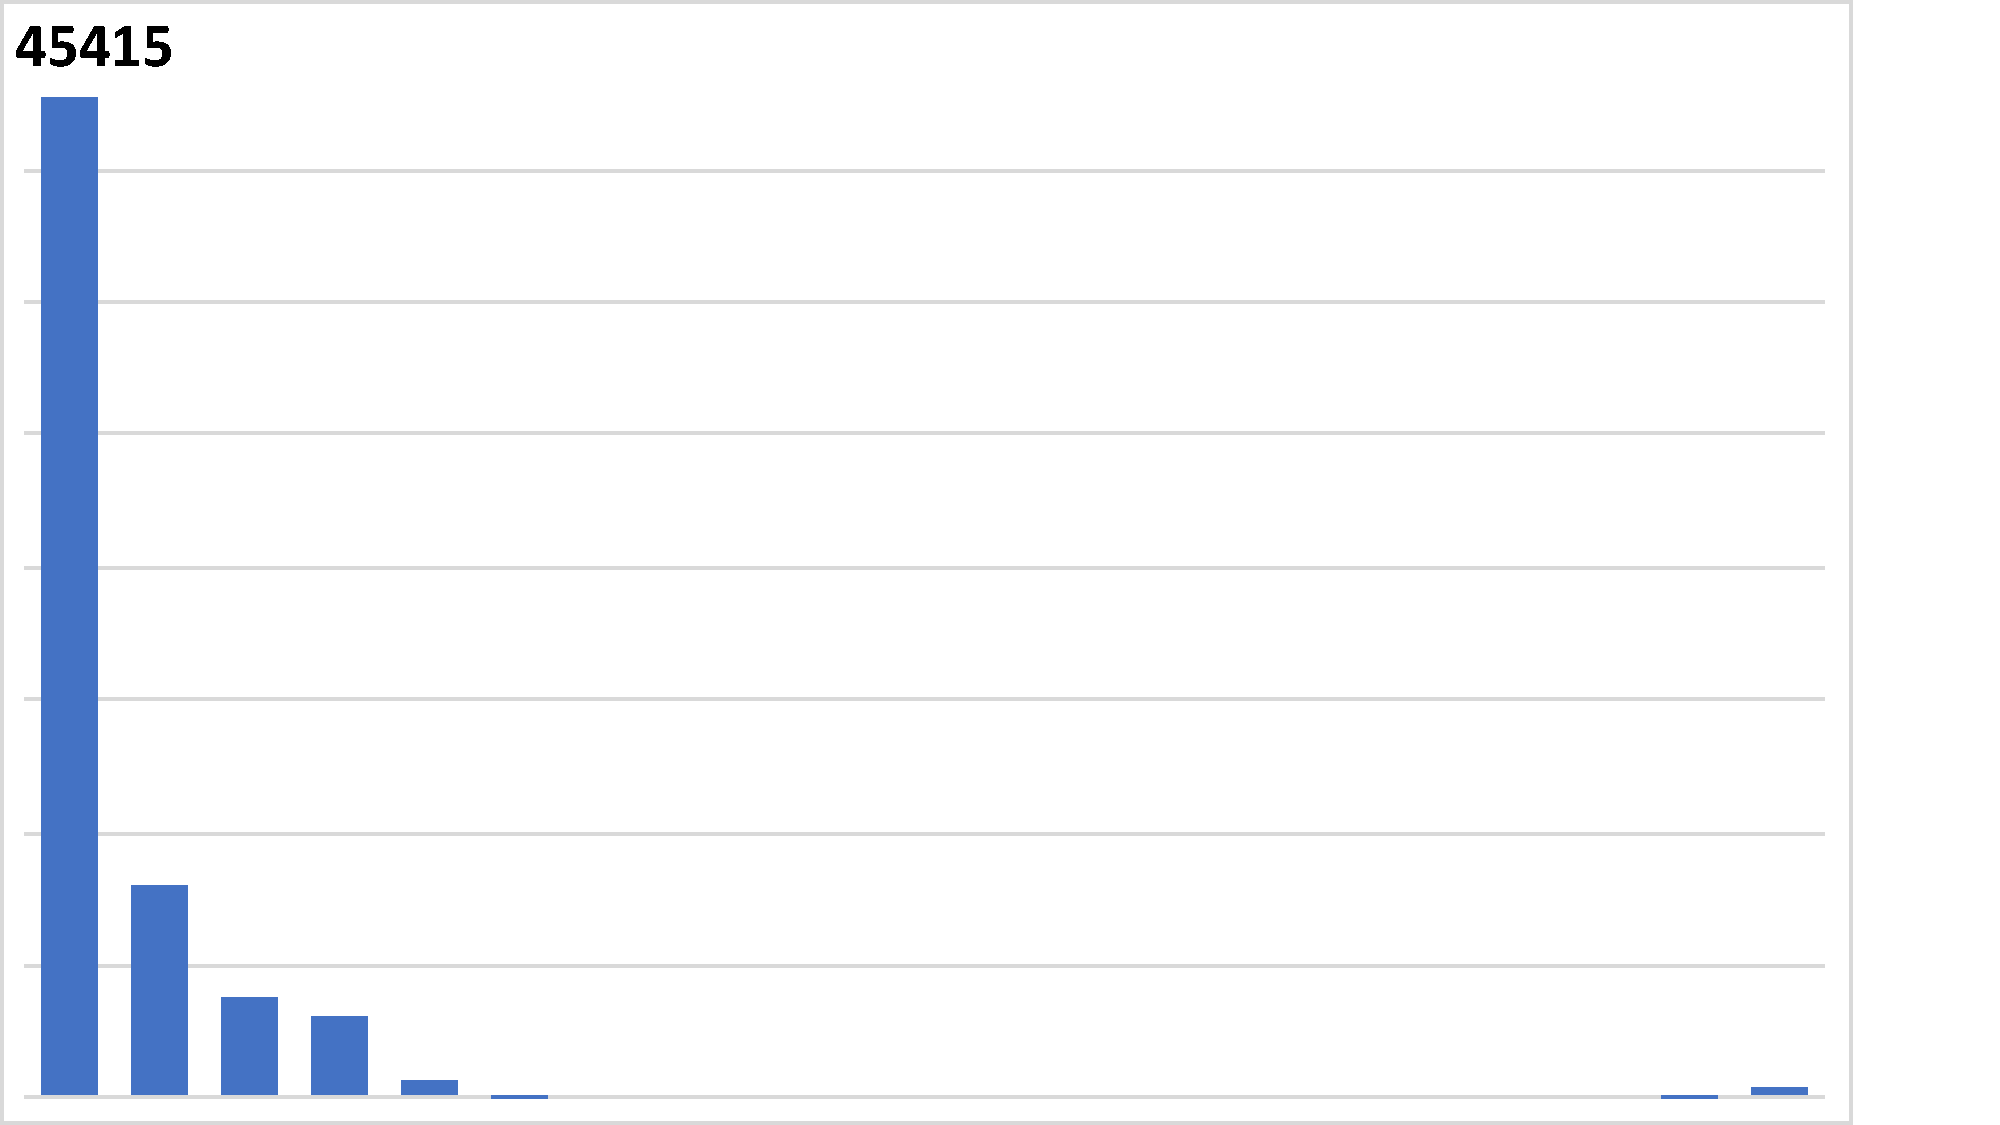
\includegraphics[width=0.7\linewidth, trim={0cm 0cm 2.5cm 0cm}, clip]{results/nyx/Eul25_AvgL2.pdf}
\caption{Eulerian 25 Avg$_{L2}$}
\end{subfigure}
\hspace{1mm}
\begin{subfigure}{0.24\textwidth}
\centering
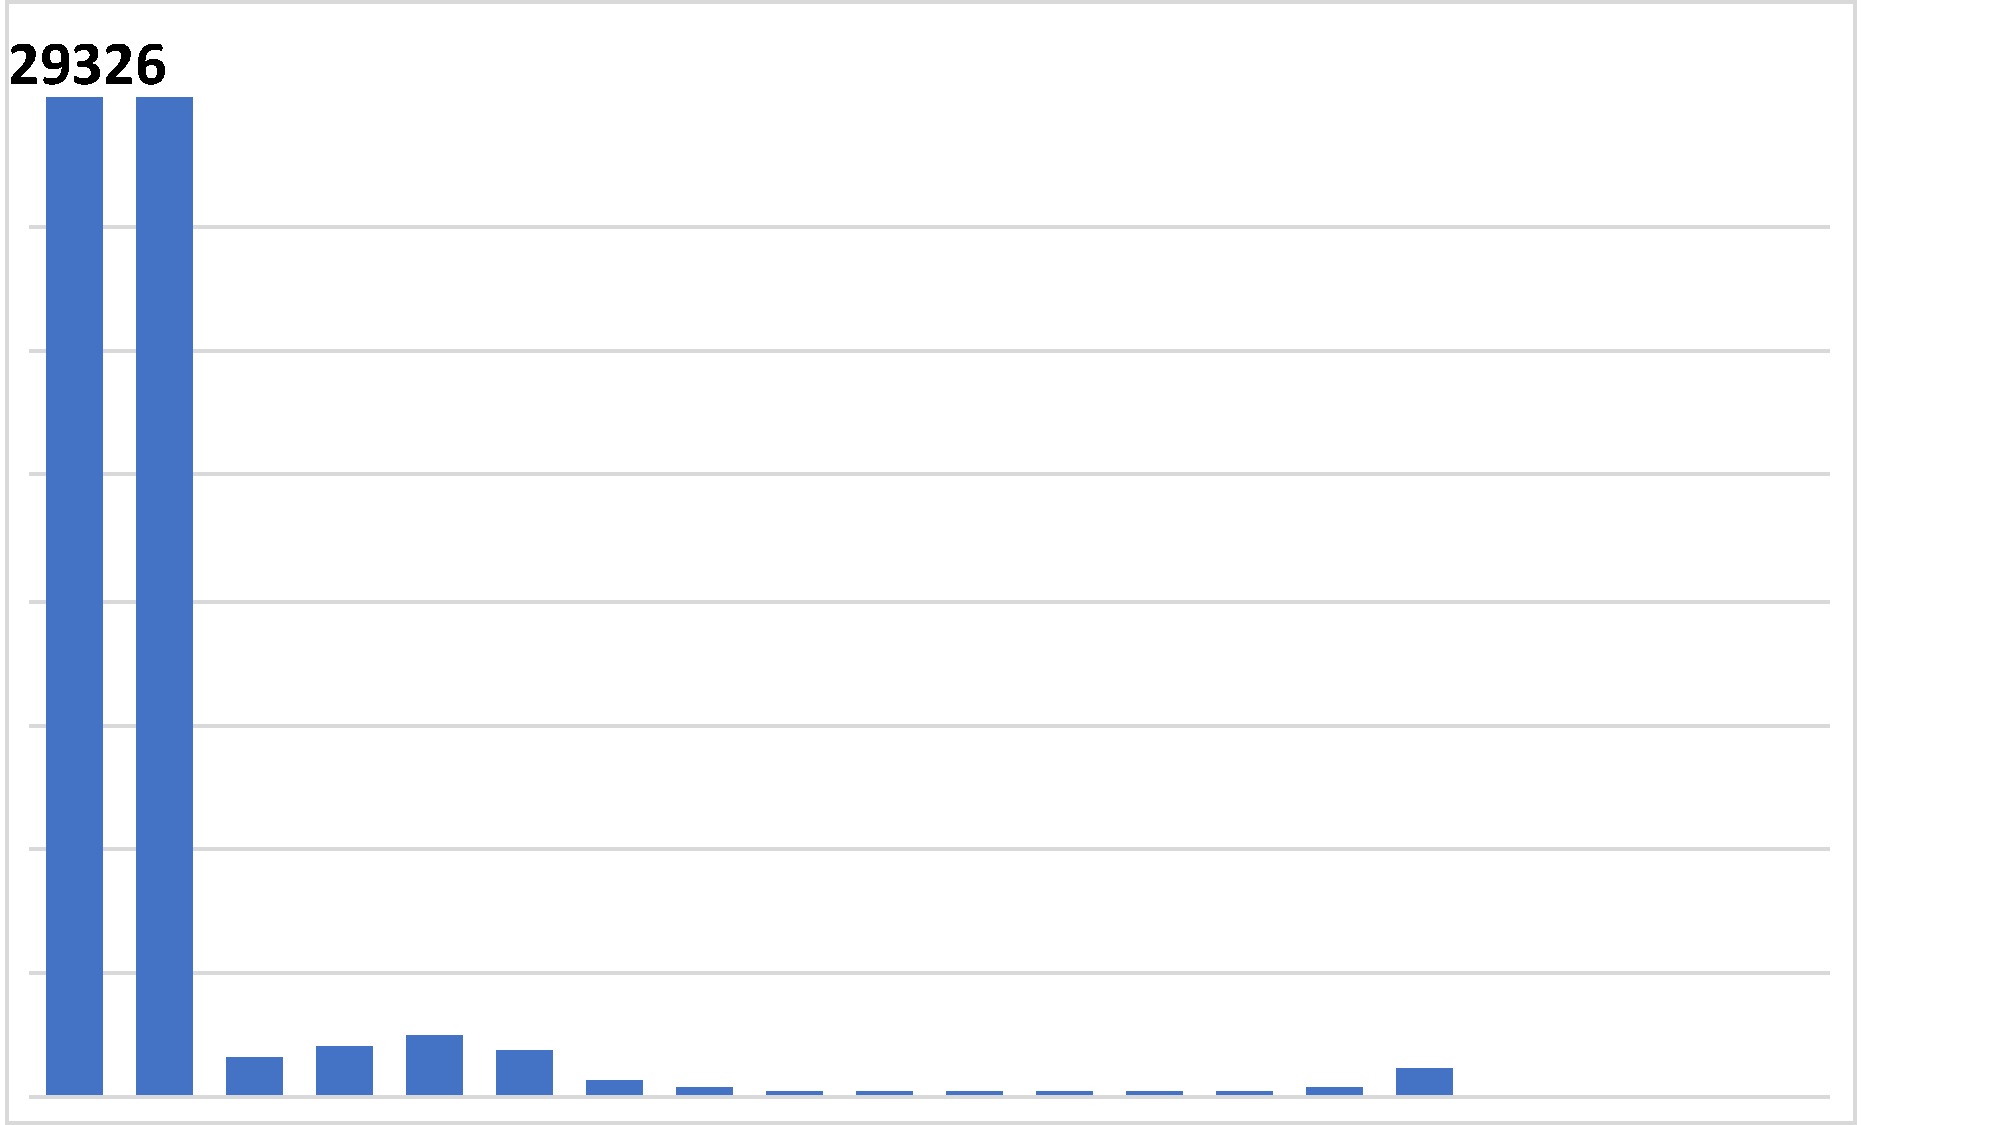
\includegraphics[width=0.7\linewidth, trim={0cm 0cm 2.5cm 0cm}, clip]{results/nyx/Eul50_AvgL2.pdf}
\caption{Eulerian 50 Avg$_{L2}$}
\end{subfigure}
\begin{subfigure}{0.24\textwidth}
\centering
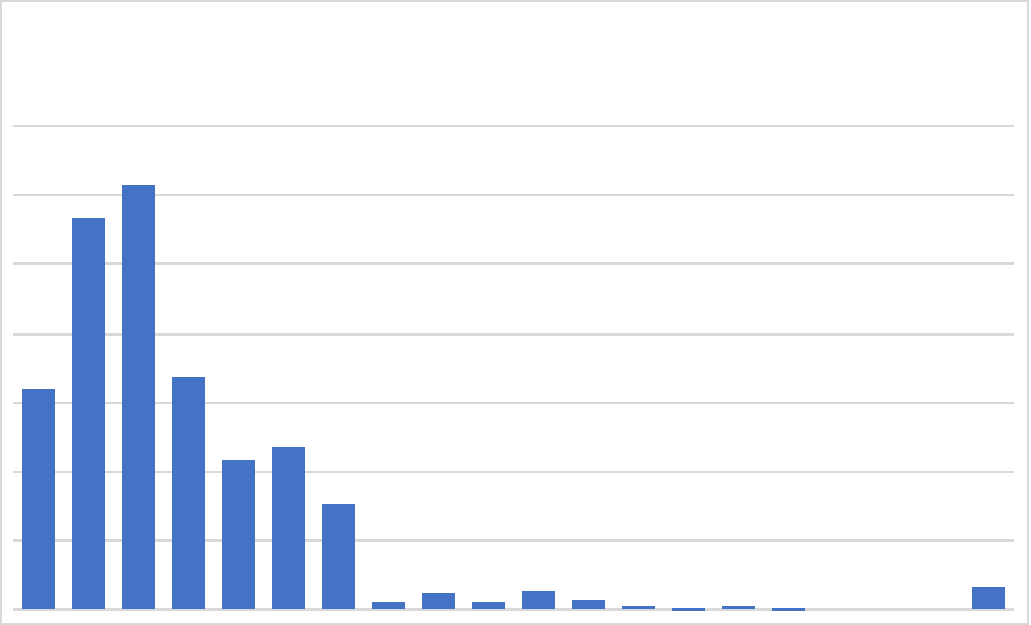
\includegraphics[width=0.7\linewidth]{results/nyx/Eul100_AvgL2.pdf}
\caption{Eulerian 100 Avg$_{L2}$}
\end{subfigure}
\hspace{1mm}
\begin{subfigure}{0.24\textwidth}
\centering
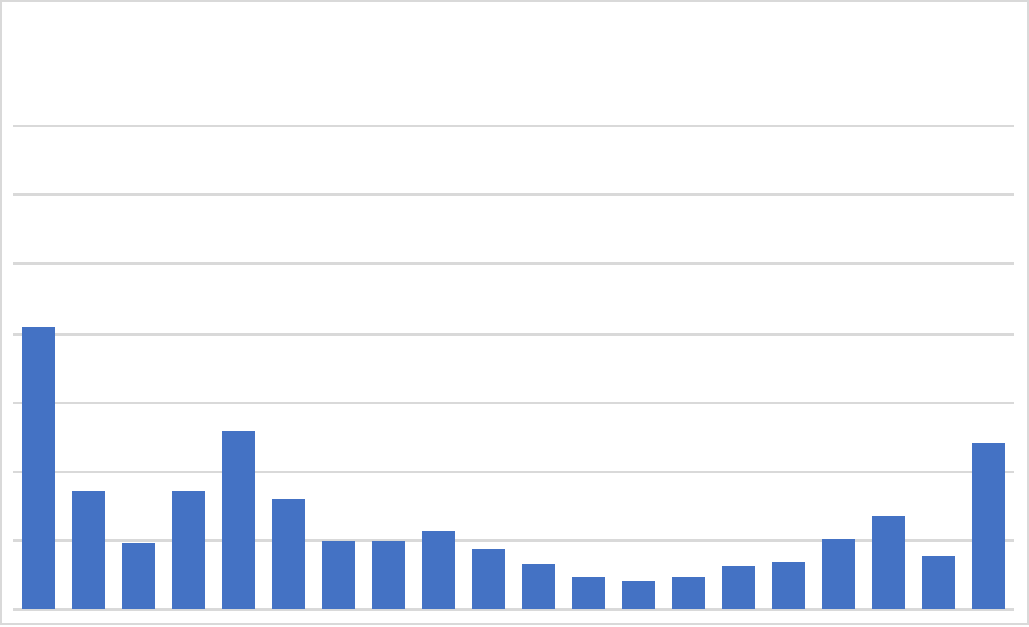
\includegraphics[width=0.7\linewidth]{results/nyx/Eul200_AvgL2.pdf}
\caption{Eulerian 200 Avg$_{L2}$}
\end{subfigure}
\begin{subfigure}{0.24\textwidth}
\centering
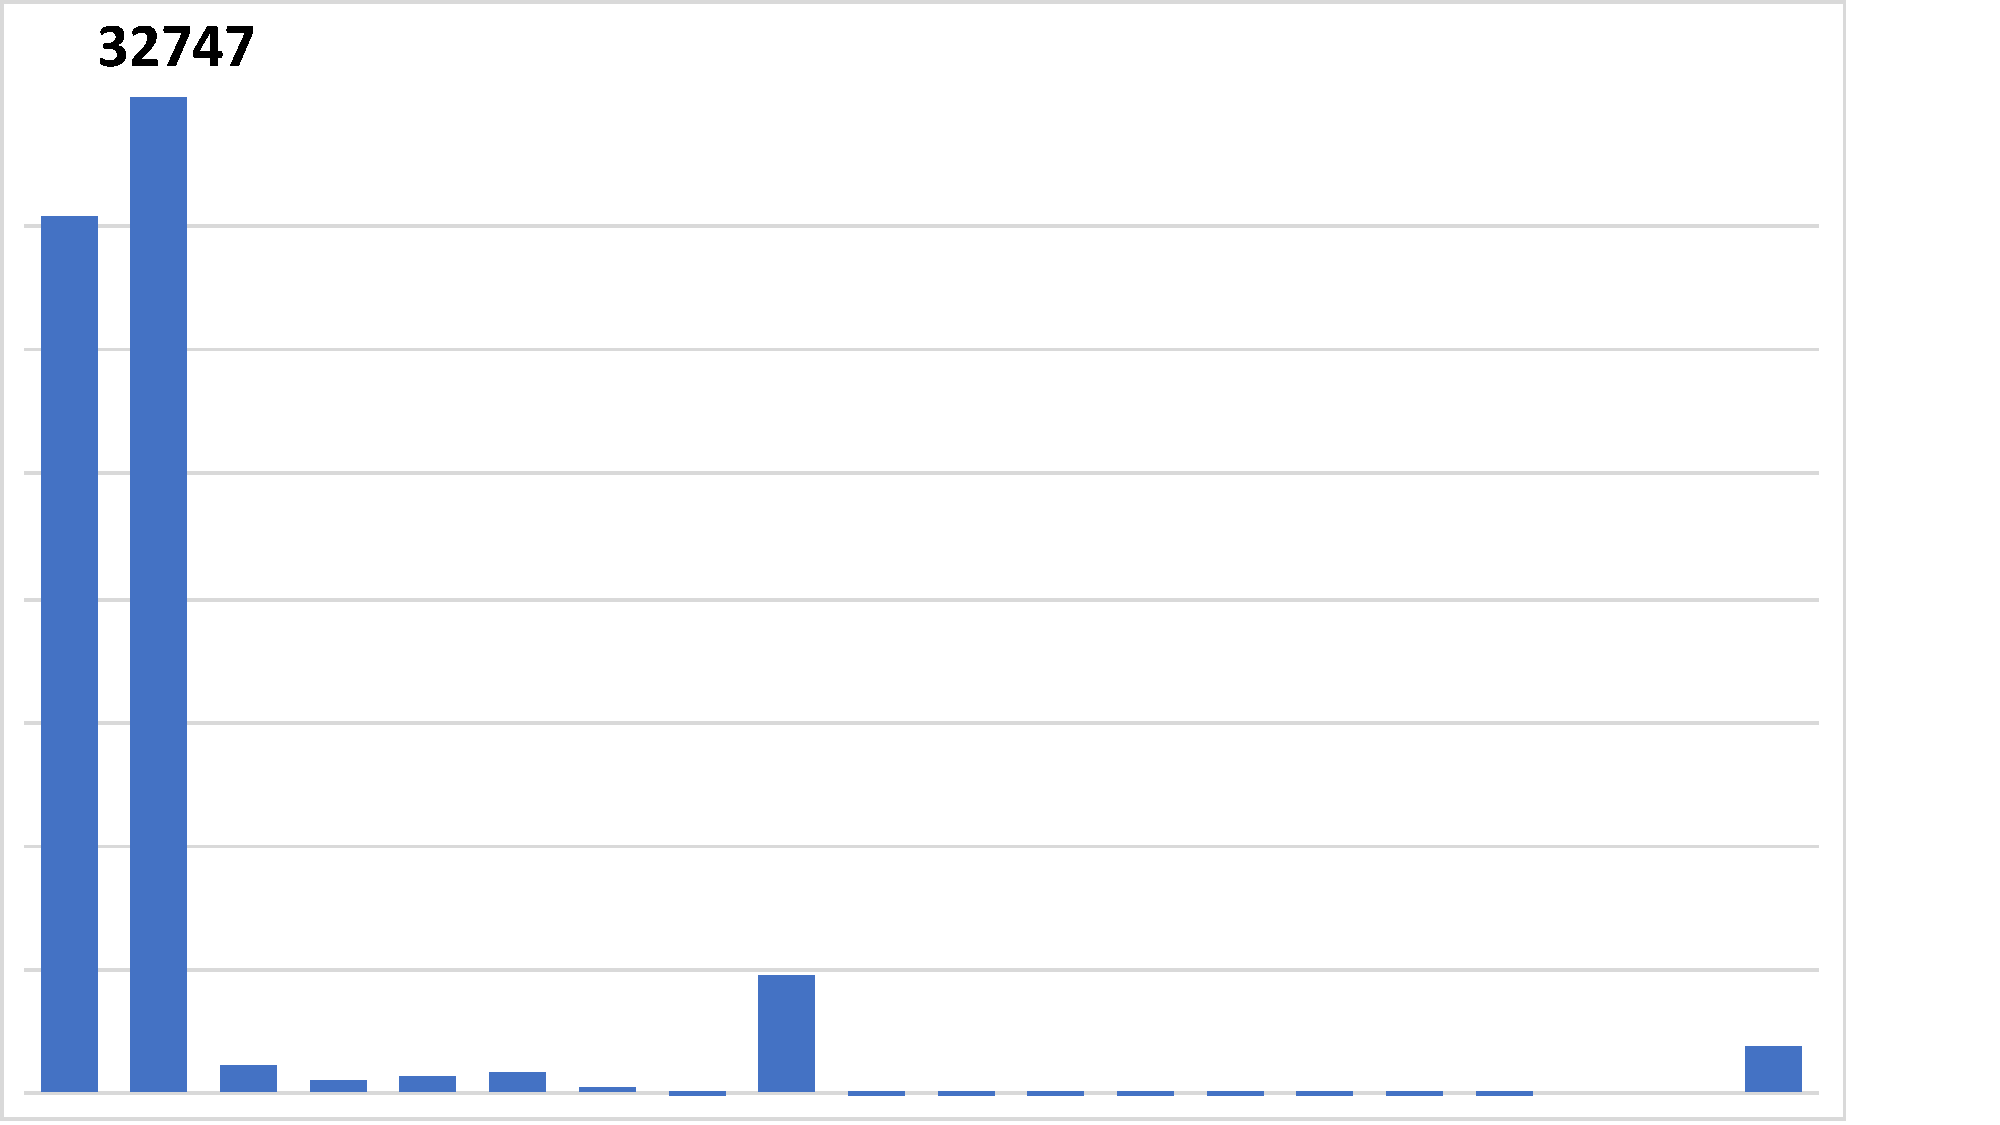
\includegraphics[width=0.7\linewidth, trim={0cm 0cm 2.5cm 0cm}, clip]{results/nyx/Eul25_Max.pdf}
\caption{Eulerian 25 Max$_{L2}$}
\end{subfigure}
\hspace{1mm}
\begin{subfigure}{0.24\textwidth}
\centering
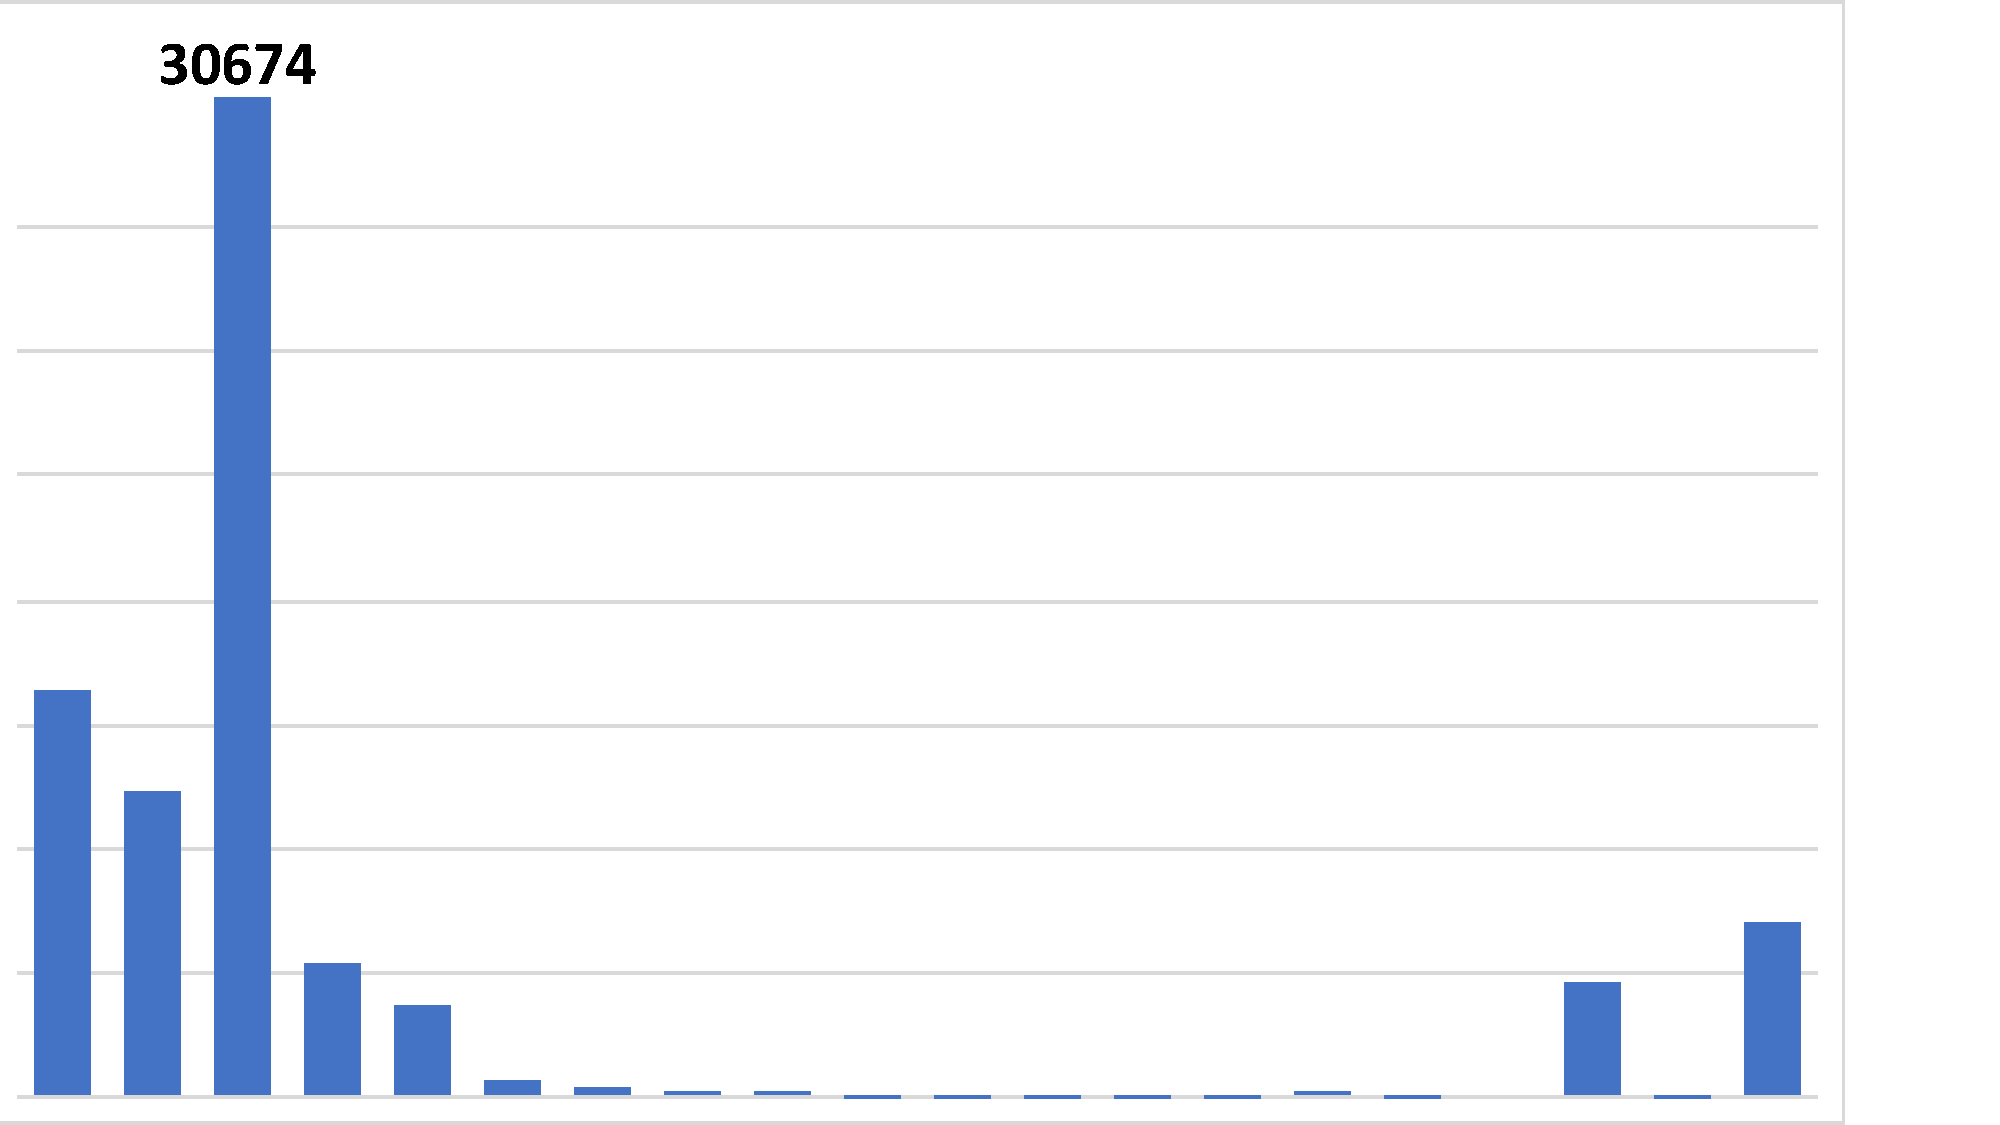
\includegraphics[width=0.7\linewidth, trim={0cm 0cm 2.5cm 0cm}, clip]{results/nyx/Eul50_Max.pdf}
\caption{Eulerian 50 Max$_{L2}$}
\end{subfigure}
\hspace{1mm}
\begin{subfigure}{0.24\textwidth}
\centering
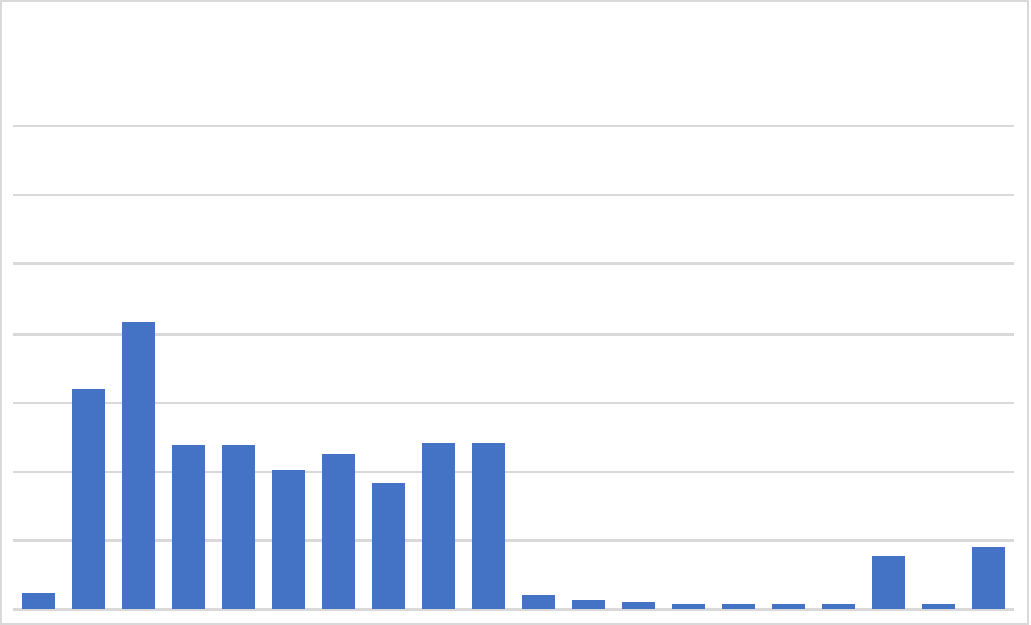
\includegraphics[width=0.7\linewidth]{results/nyx/Eul100_Max.pdf}
\caption{Eulerian 100 Max$_{L2}$}
\end{subfigure}
\hspace{1mm}
\begin{subfigure}{0.24\textwidth}
\centering
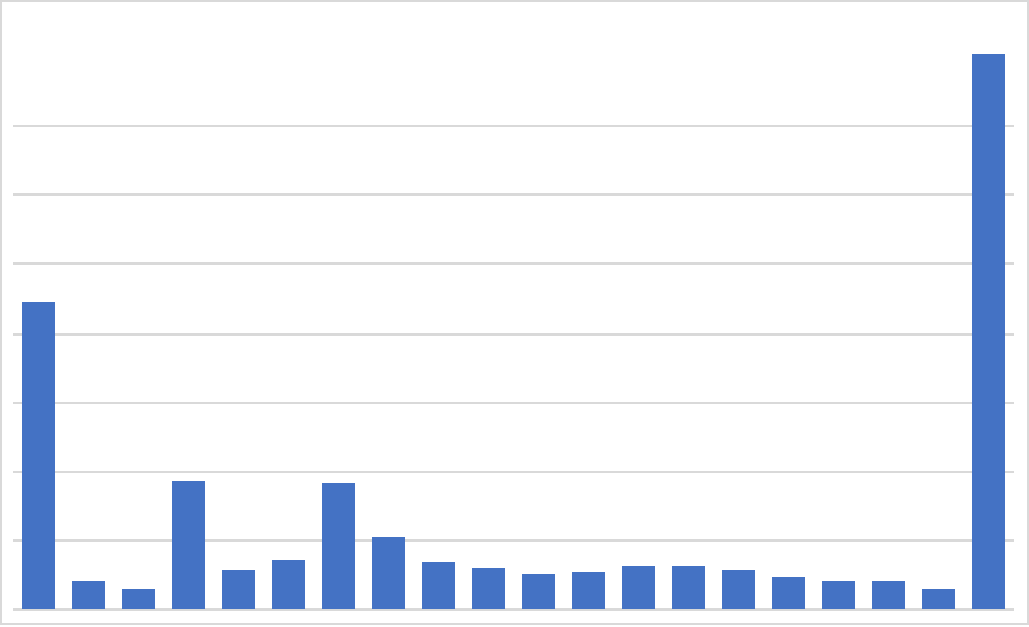
\includegraphics[width=0.7\linewidth]{results/nyx/Eul200_Max.pdf}
\caption{Eulerian 200 Max$_{L2}$}
\end{subfigure}
\hspace{1mm}
\begin{subfigure}{0.24\textwidth}
\centering
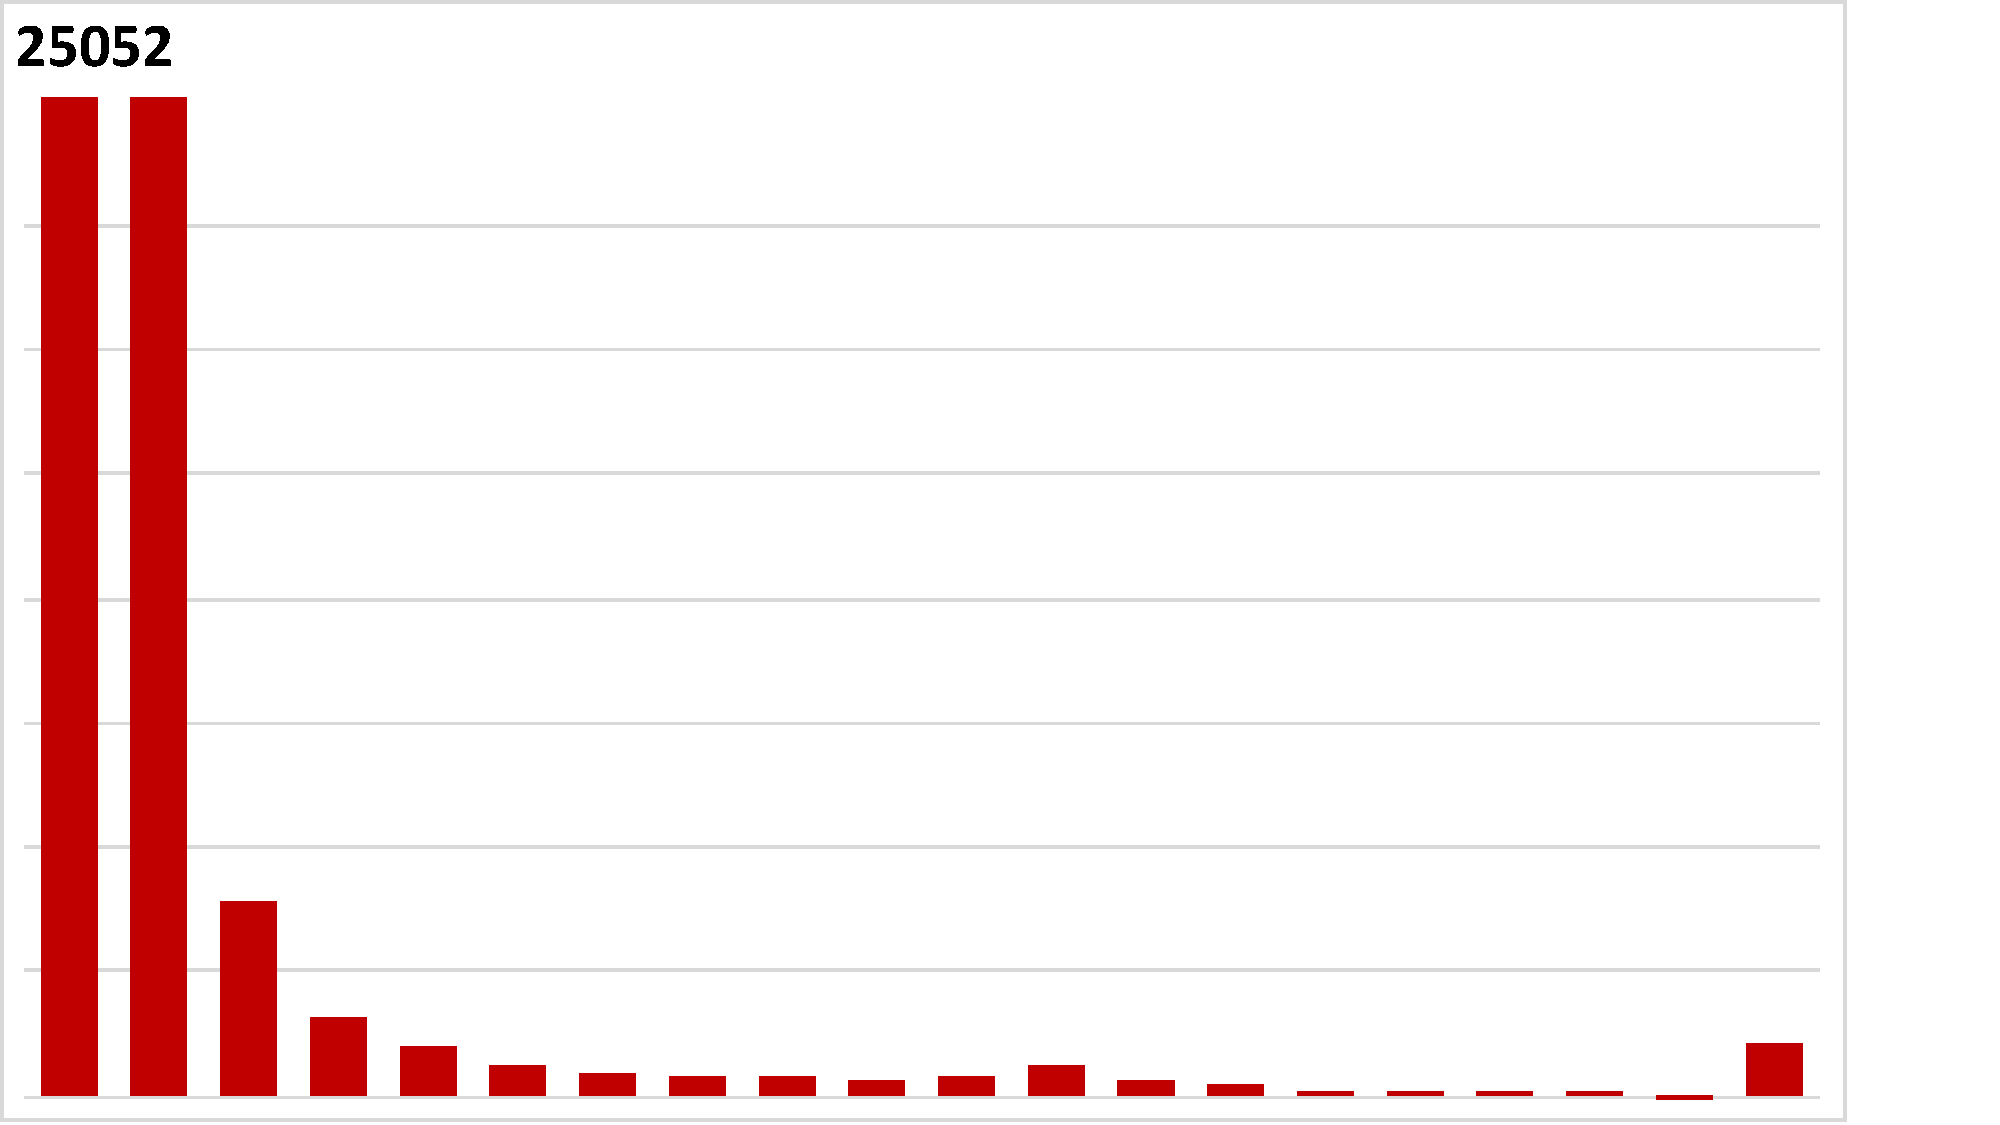
\includegraphics[width=0.7\linewidth, trim={0cm 0cm 2.5cm 0cm}, clip]{results/nyx/Lag25_1_AvgL2.pdf}
\caption{Lagrangian 25 1:1 Avg$_{L2}$}
\end{subfigure}
\hspace{1mm}
\begin{subfigure}{0.24\textwidth}
\centering
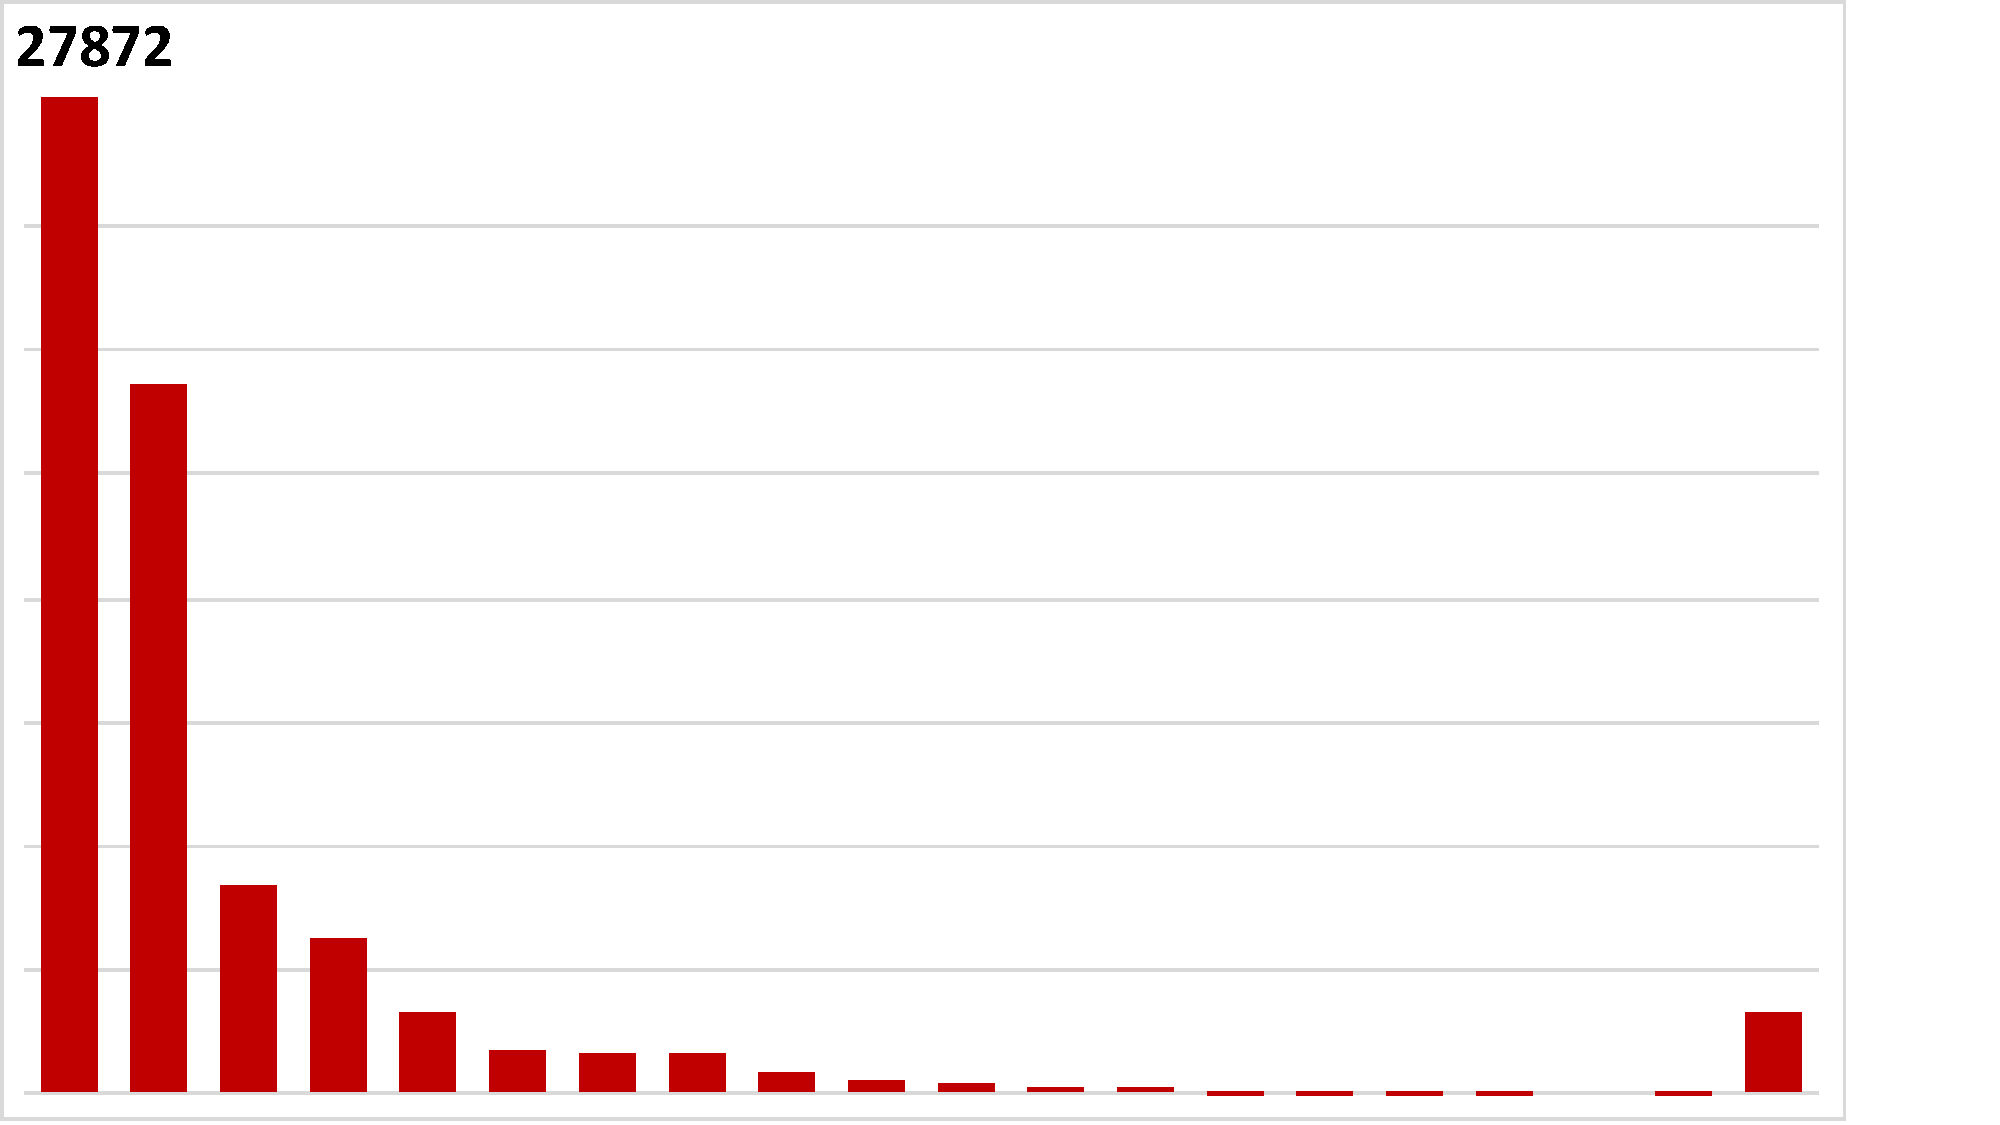
\includegraphics[width=0.7\linewidth, trim={0cm 0cm 2.5cm 0cm}, clip]{results/nyx/Lag50_1_AvgL2.pdf}
\caption{Lagrangian 50 1:1 Avg$_{L2}$}
\end{subfigure}
\hspace{1mm}
\begin{subfigure}{0.24\textwidth}
\centering
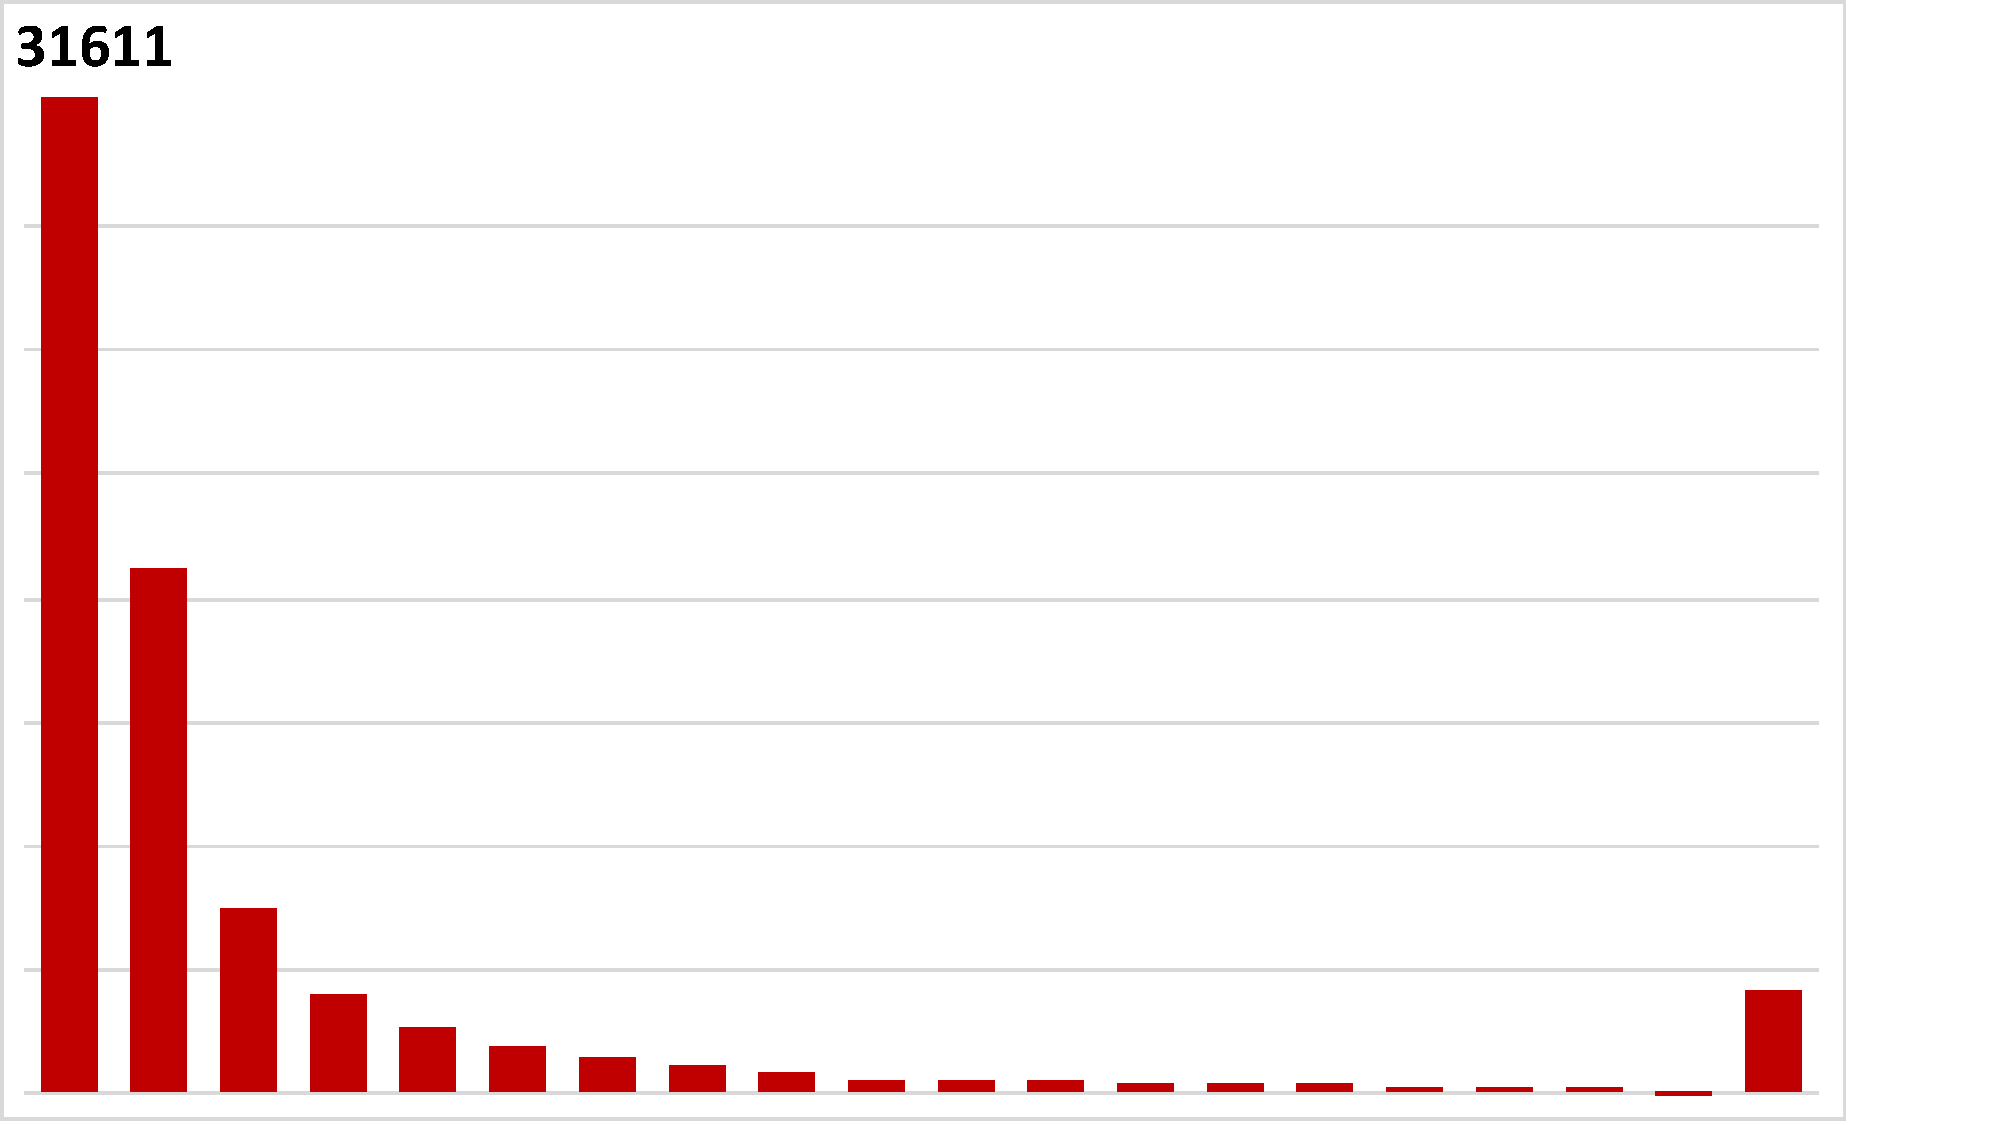
\includegraphics[width=0.7\linewidth, trim={0cm 0cm 2.5cm 0cm}, clip]{results/nyx/Lag100_1_AvgL2.pdf}
\caption{Lagrangian 100 1:1 Avg$_{L2}$}
\end{subfigure}
\hspace{1mm}
\begin{subfigure}{0.24\textwidth}
\centering
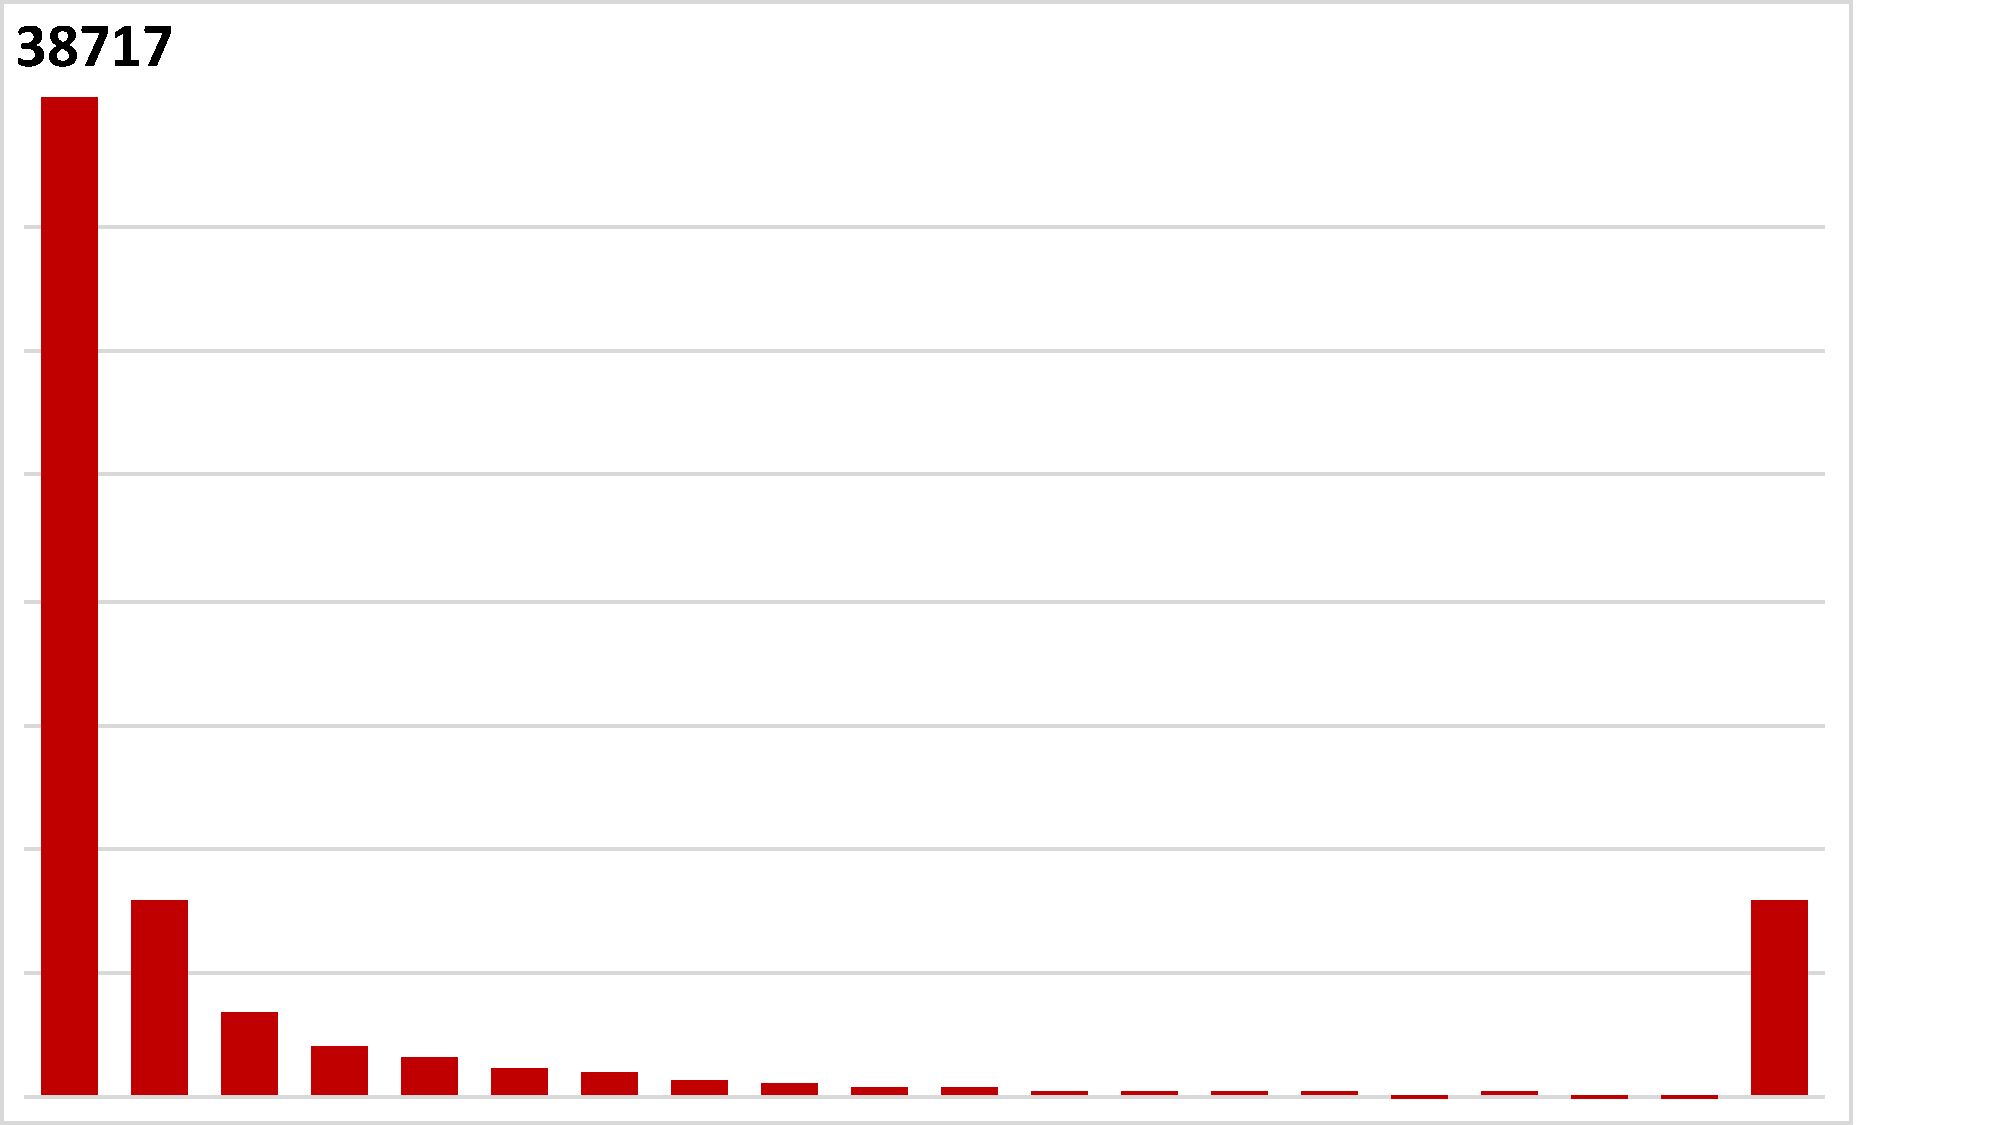
\includegraphics[width=0.7\linewidth, trim={0cm 0cm 2.5cm 0cm}, clip]{results/nyx/Lag200_1_AvgL2.pdf}
\caption{Lagrangian 200 1:1 Avg$_{L2}$}
\end{subfigure}
\hspace{1mm}
\begin{subfigure}{0.24\textwidth}
\centering
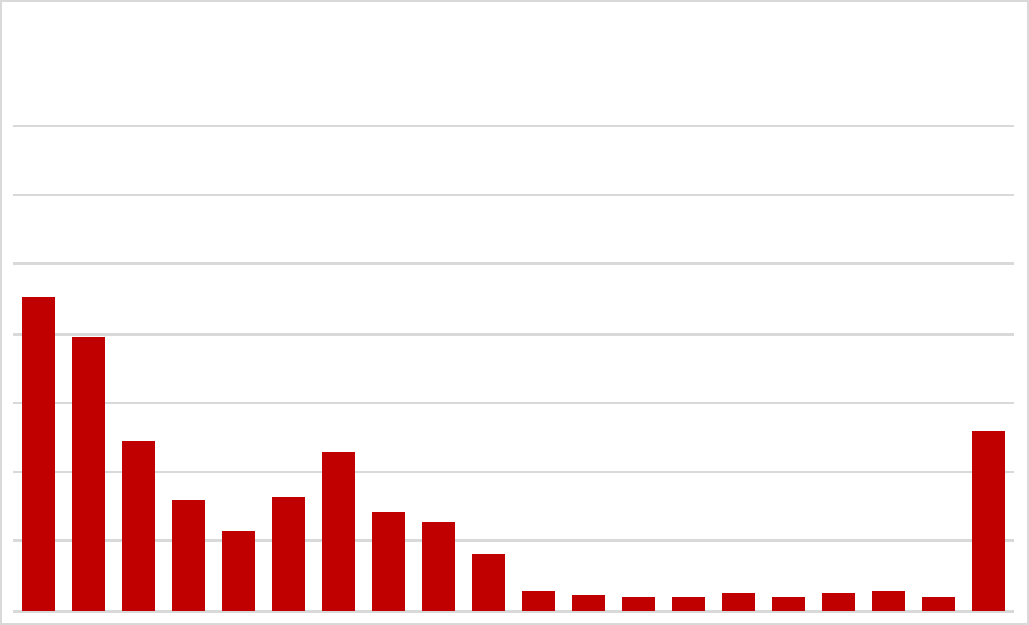
\includegraphics[width=0.7\linewidth]{results/nyx/Lag25_1_Max.pdf}
\caption{Lagrangian 25 1:1 Max$_{L2}$}
\end{subfigure}
\hspace{1mm}
\begin{subfigure}{0.24\textwidth}
\centering
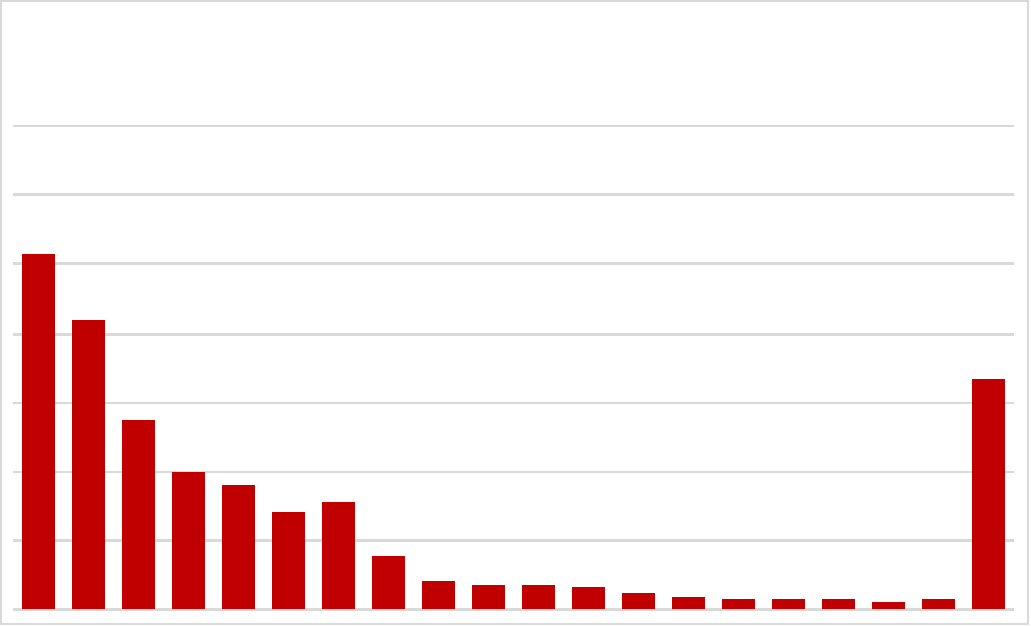
\includegraphics[width=0.7\linewidth]{results/nyx/Lag50_1_Max.pdf}
\caption{Lagrangian 50 1:1 Max$_{L2}$}
\end{subfigure}
\hspace{1mm}
\begin{subfigure}{0.24\textwidth}
\centering
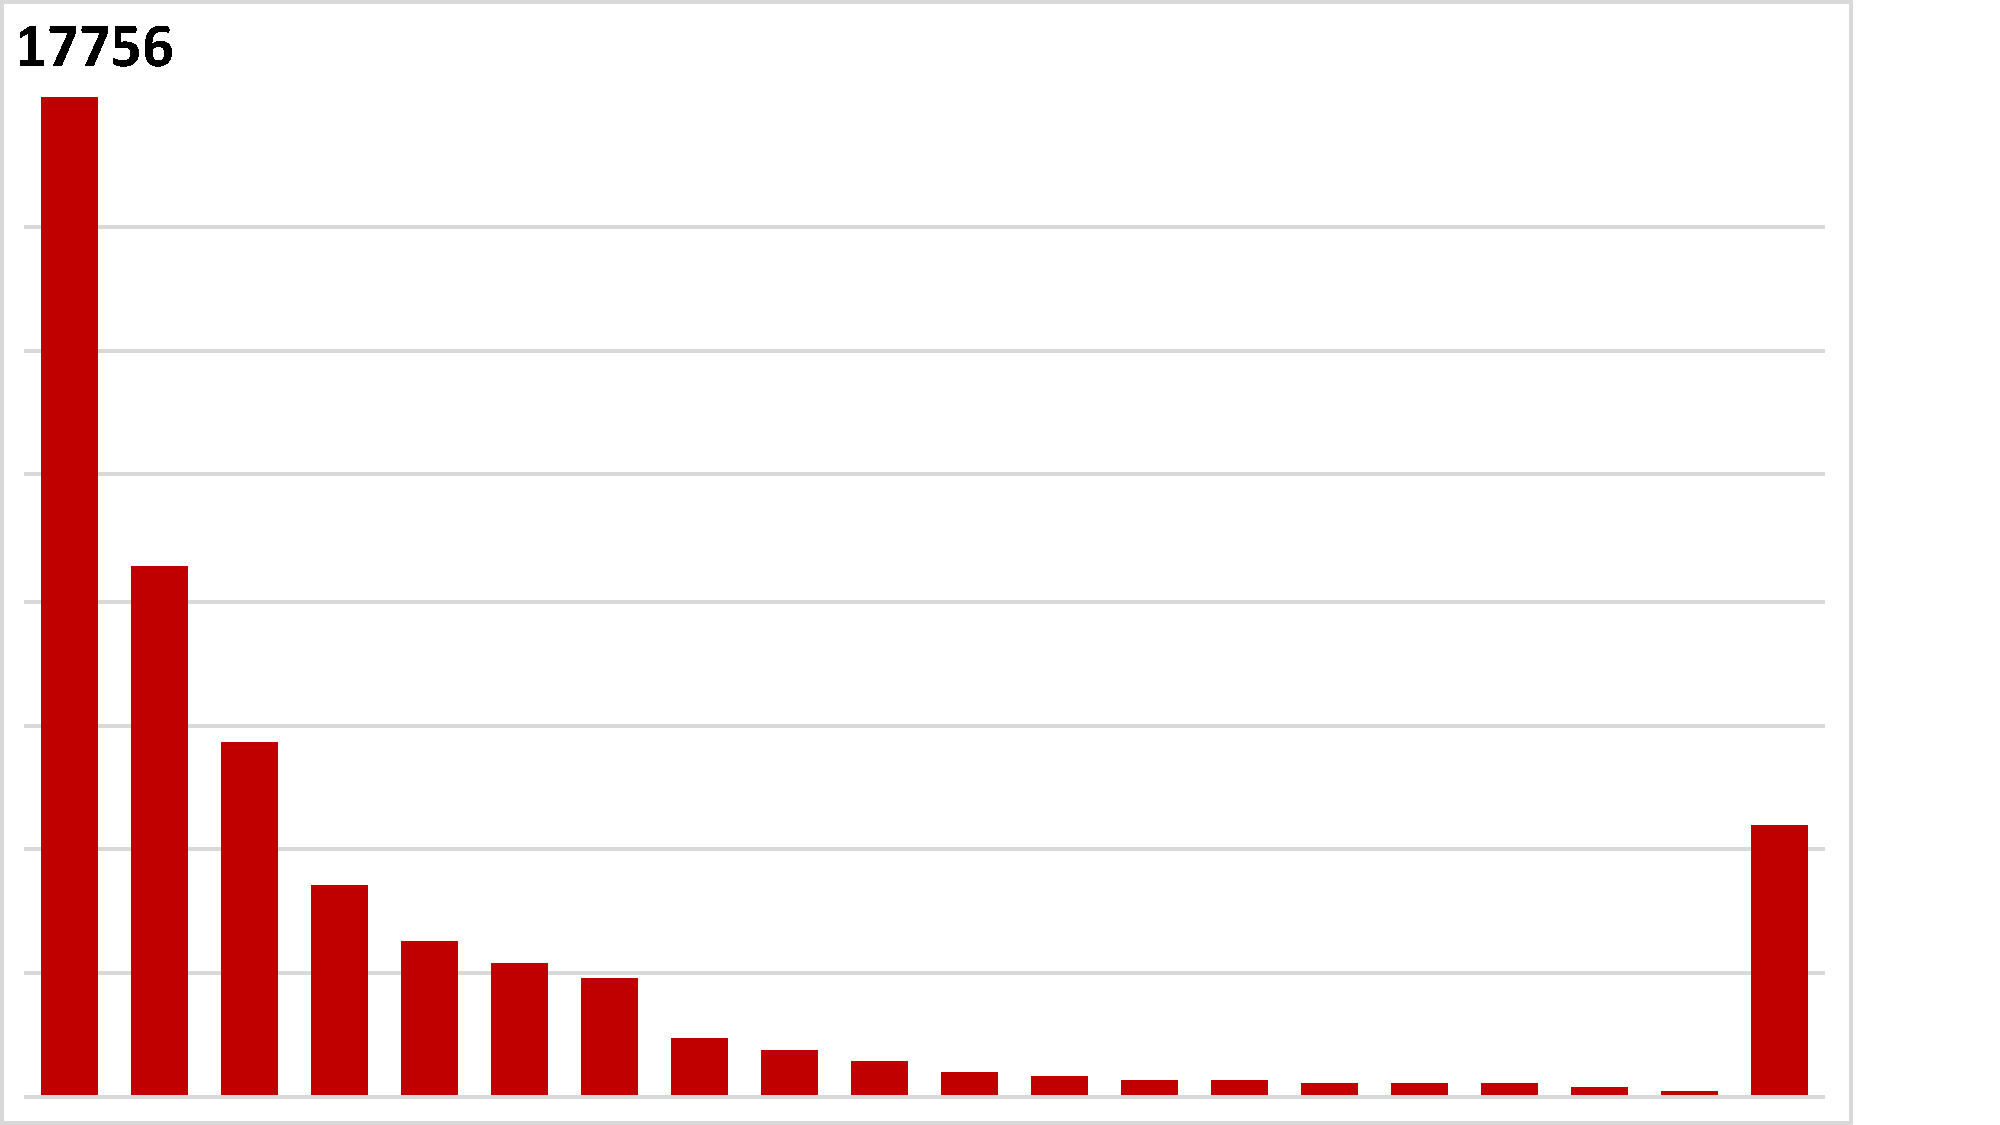
\includegraphics[width=0.7\linewidth, trim={0cm 0cm 2.5cm 0cm}, clip]{results/nyx/Lag100_1_Max.pdf}
\caption{Lagrangian 100 1:1 Max$_{L2}$}
\end{subfigure}
\hspace{1mm}
\begin{subfigure}{0.24\textwidth}
\centering
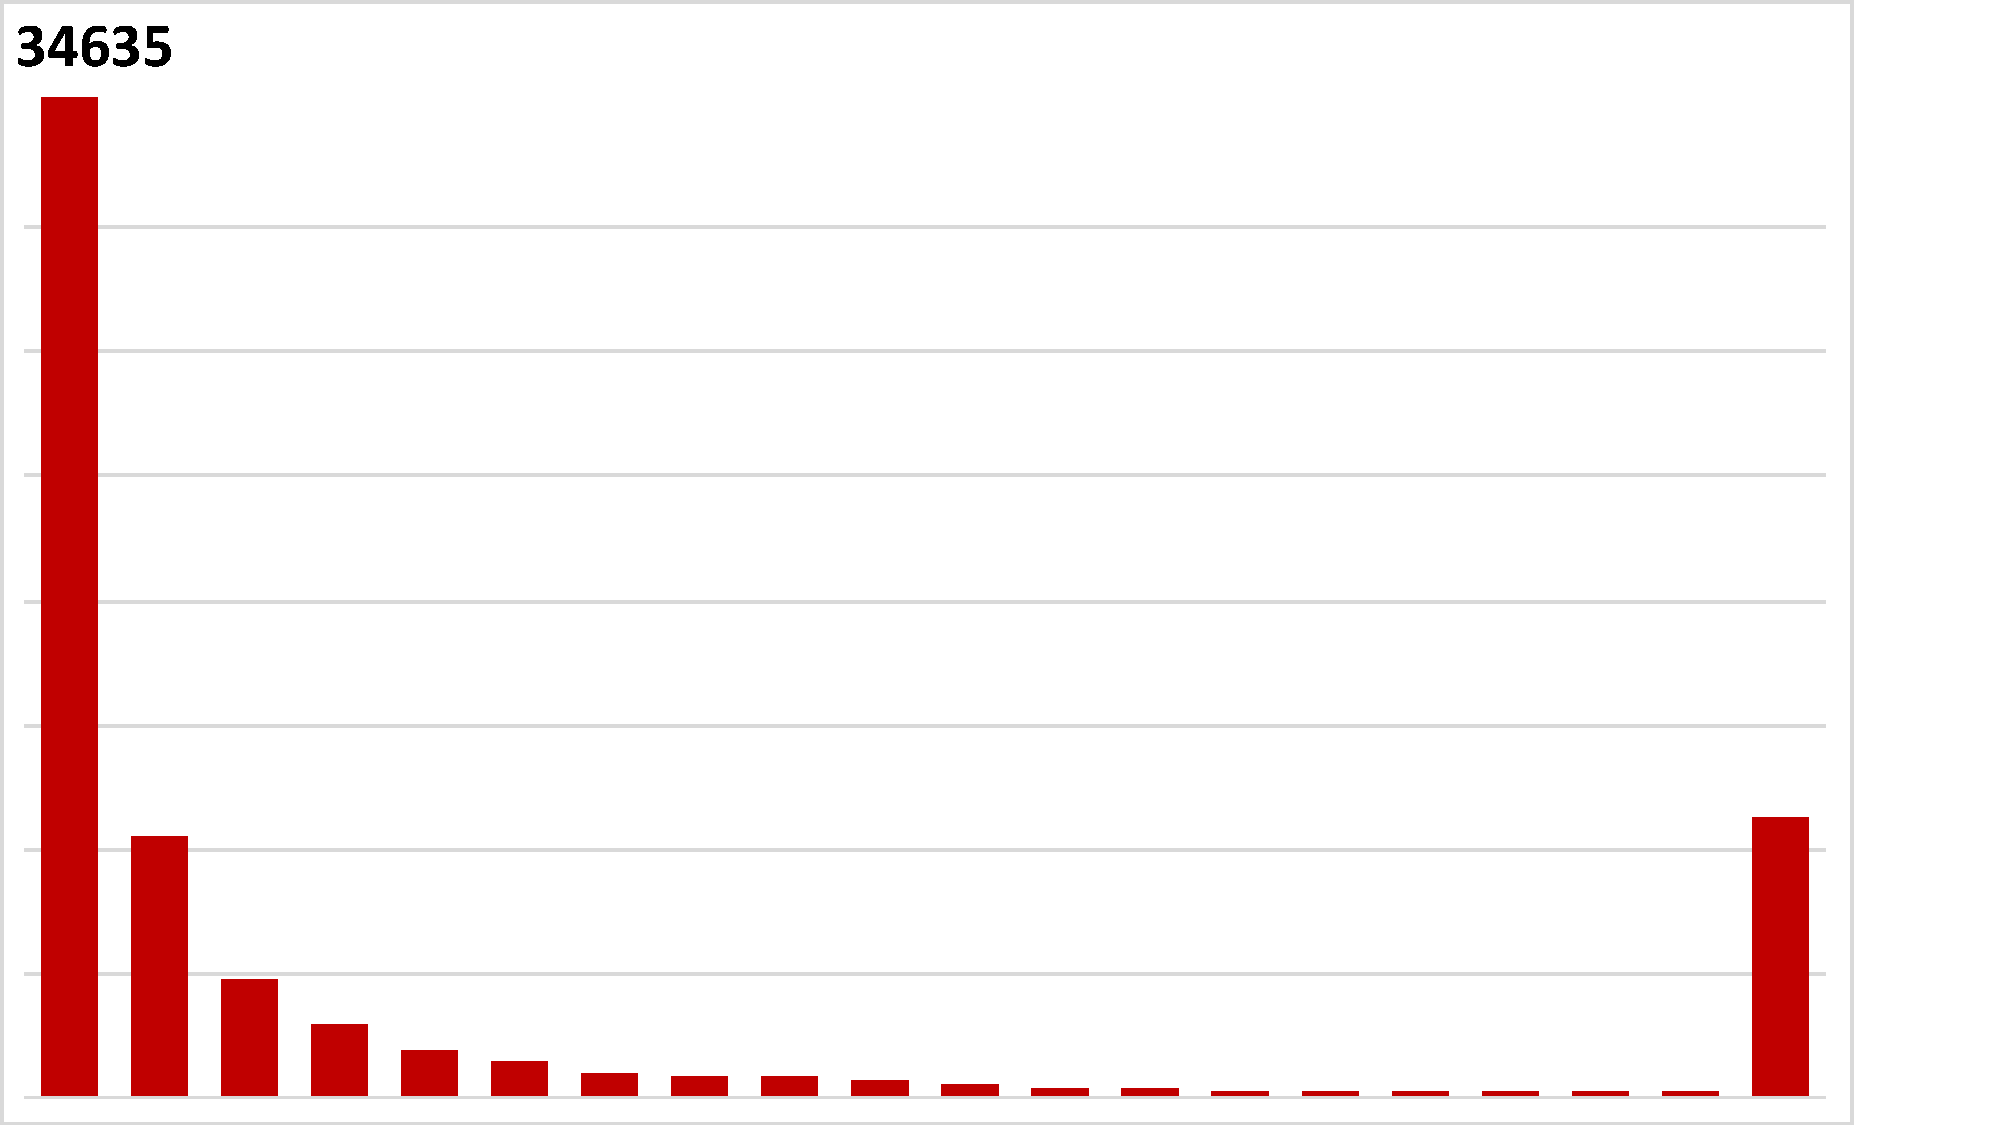
\includegraphics[width=0.7\linewidth, trim={0cm 0cm 2.5cm 0cm}, clip]{results/nyx/Lag200_1_Max.pdf}
\caption{Lagrangian 200 1:1 Max$_{L2}$}
\end{subfigure}
%\begin{subfigure}{0.24\textwidth}
%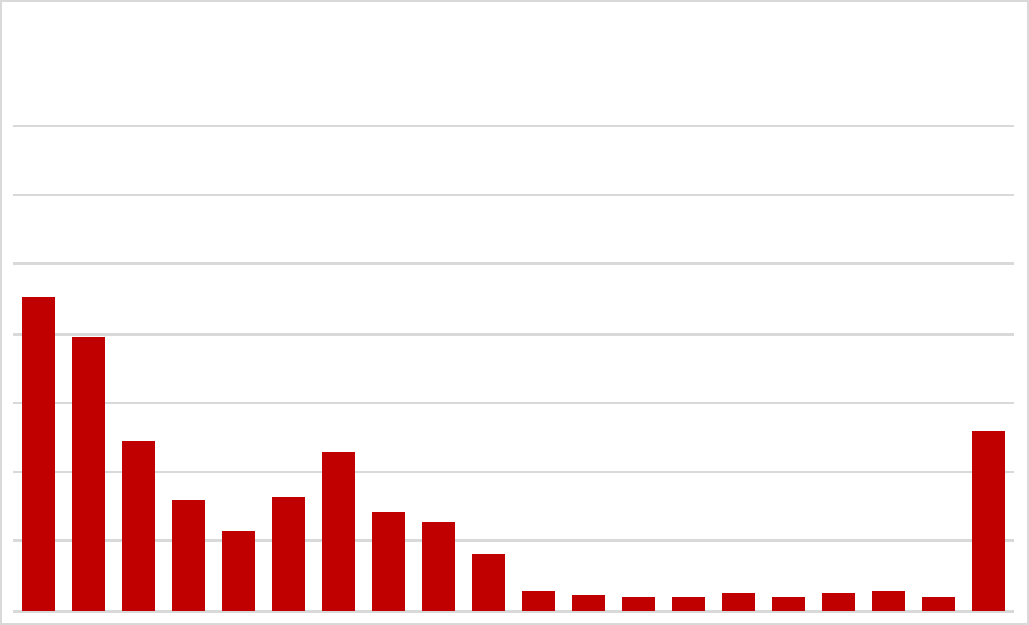
\includegraphics[width=0.8\linewidth]{results/nyx/Lag25_1_Max.pdf}
%\caption{Lagrangian 25 1:1 Max$_{L2}$}
%\end{subfigure}
%\hspace{1mm}
%\begin{subfigure}{0.20\textwidth}
%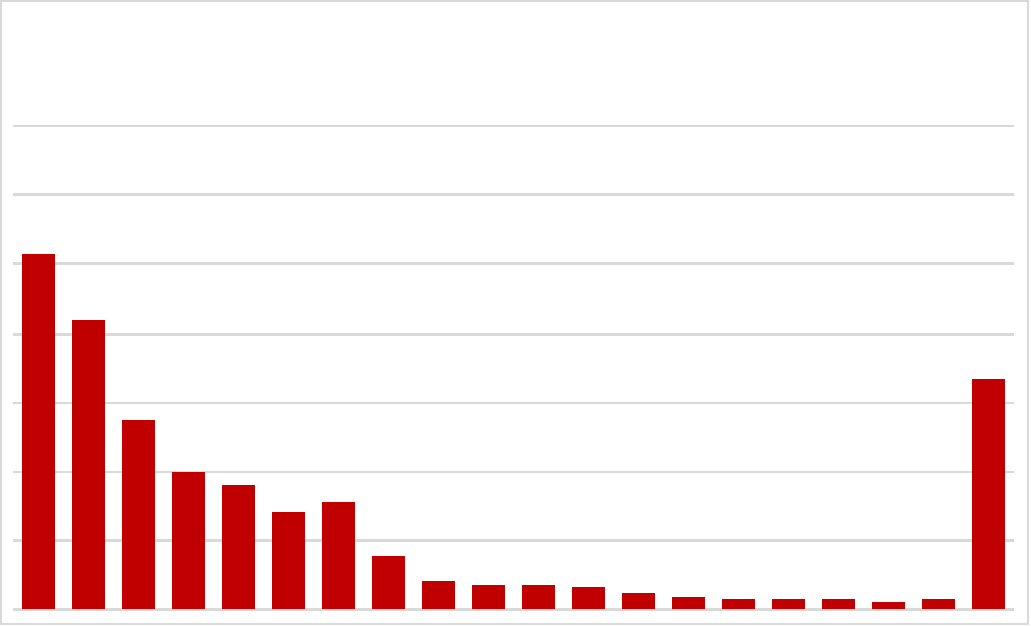
\includegraphics[width=1\linewidth]{results/nyx/Lag50_1_Max.pdf}
%\caption{Lagrangian 50 1:1 Max$_{L2}$}
%\end{subfigure}
%\begin{subfigure}{0.20\textwidth}
%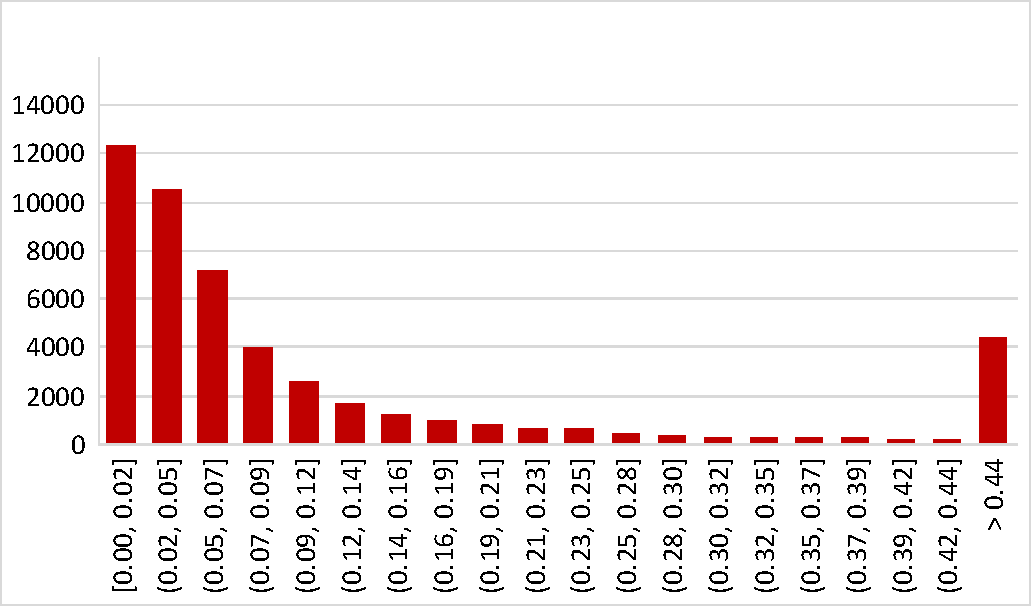
\includegraphics[width=1\linewidth]{results/nyx/Lag100_8_AvgL2.pdf}
%\caption{Lagrangian 100 1:8 Avg$_{L2}$}
%\end{subfigure}
%\hspace{1mm}
%\begin{subfigure}{0.20\textwidth}
%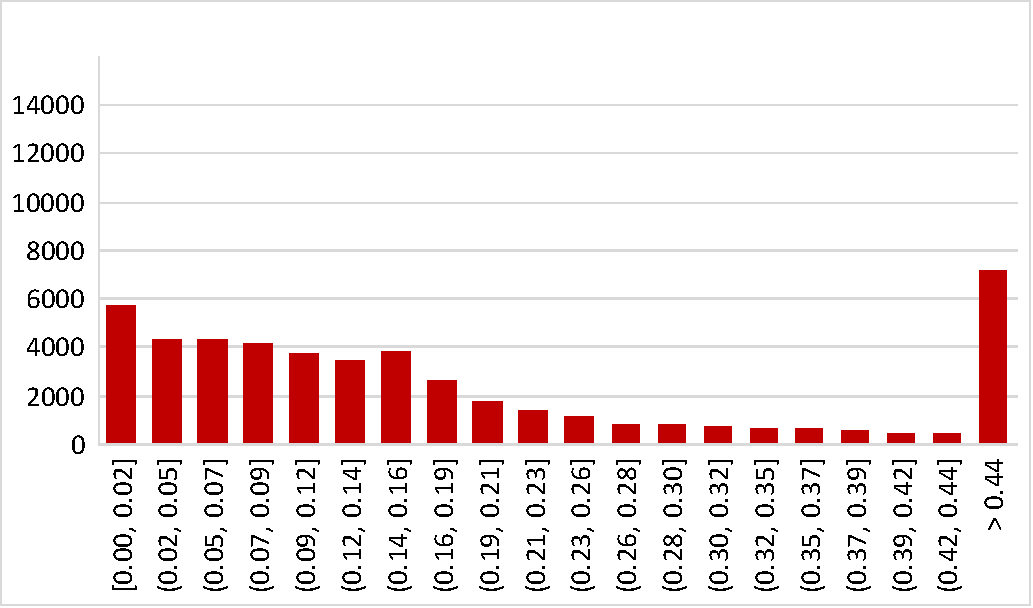
\includegraphics[width=1\linewidth]{results/nyx/Lag100_27_AvgL2.pdf}
%\caption{Lagrangian 100 1:27 Avg$_{L2}$}
%\end{subfigure}
%\begin{subfigure}{0.20\textwidth}
%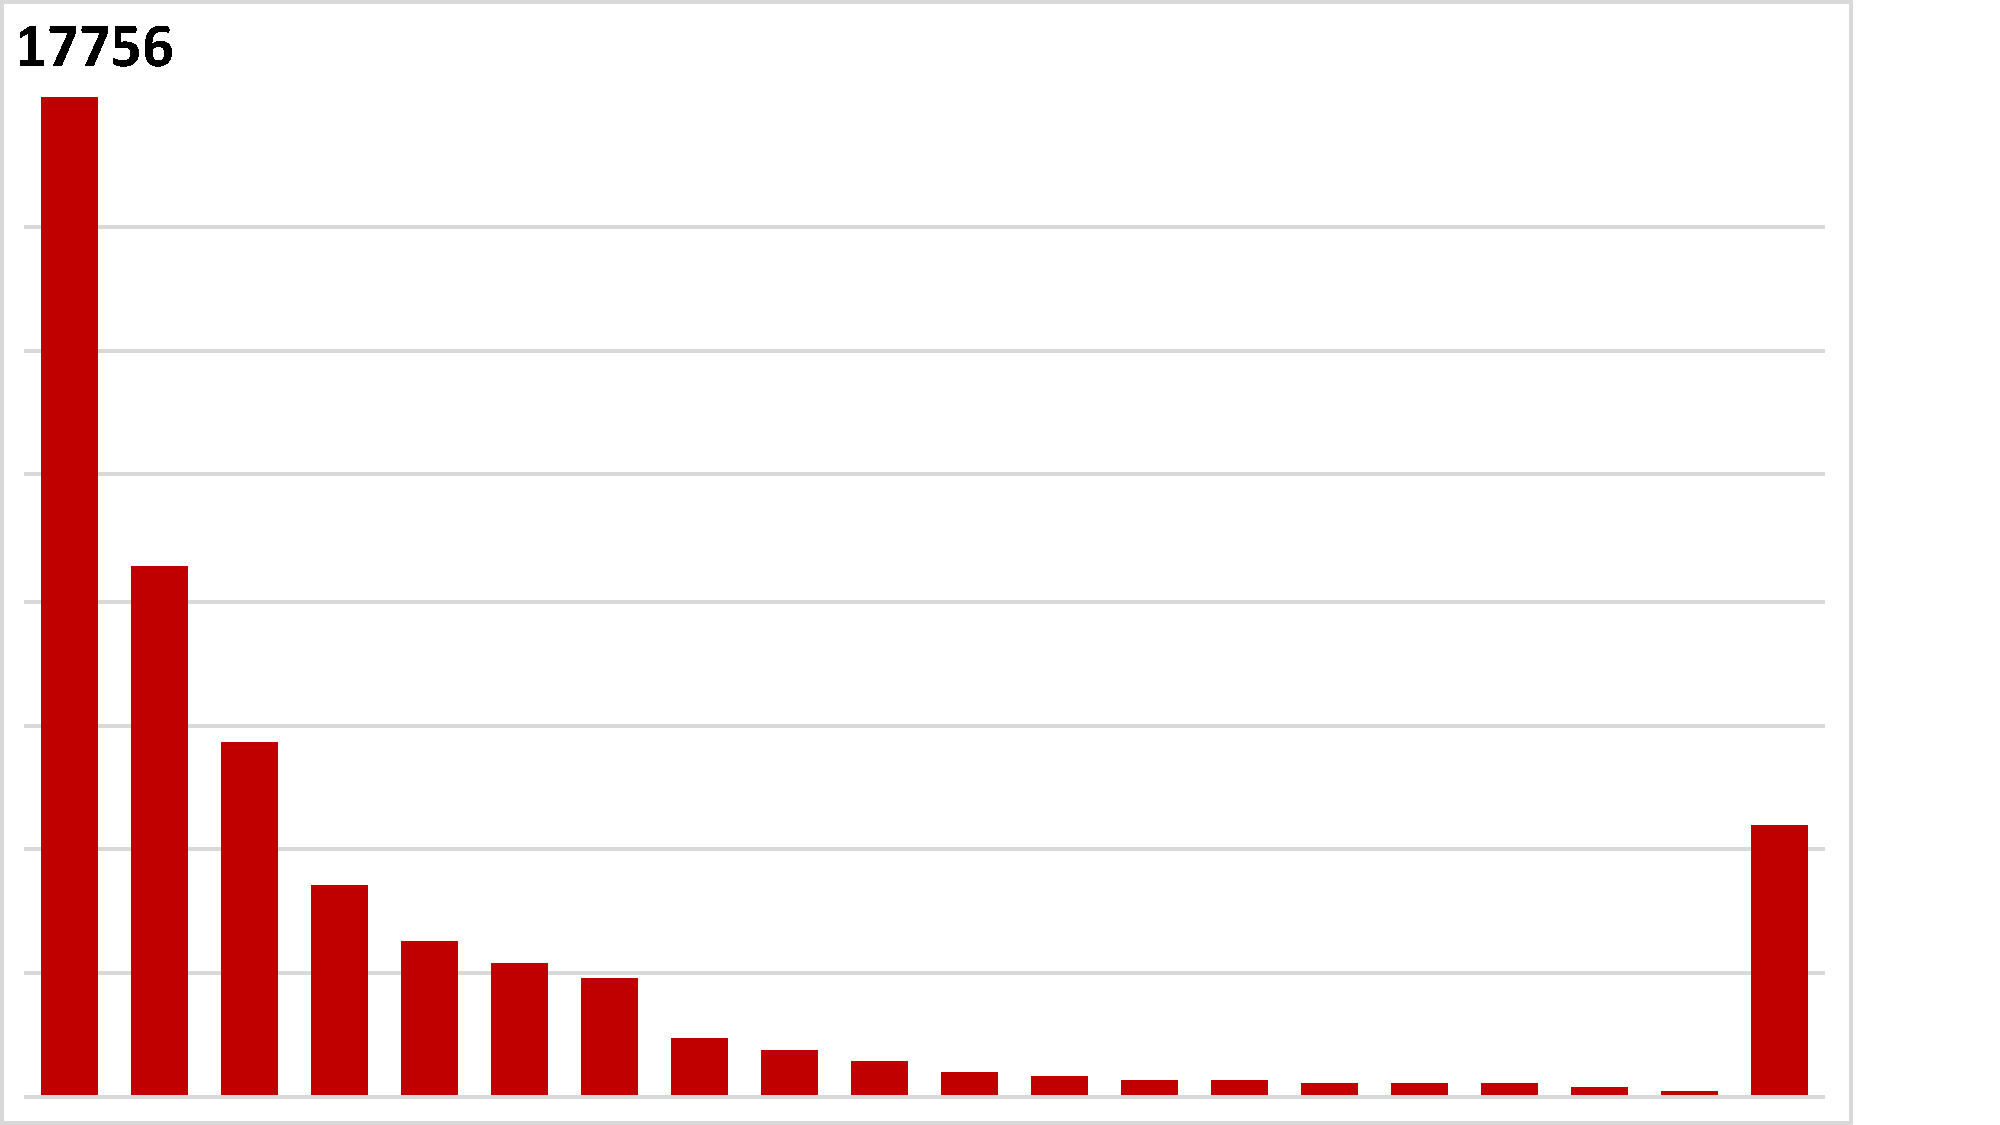
\includegraphics[width=1\linewidth]{results/nyx/Lag100_1_Max.pdf}
%\caption{Lagrangian 100 1:1 Max$_{L2}$}
%\end{subfigure}
%\hspace{1mm}
%\begin{subfigure}{0.20\textwidth}
%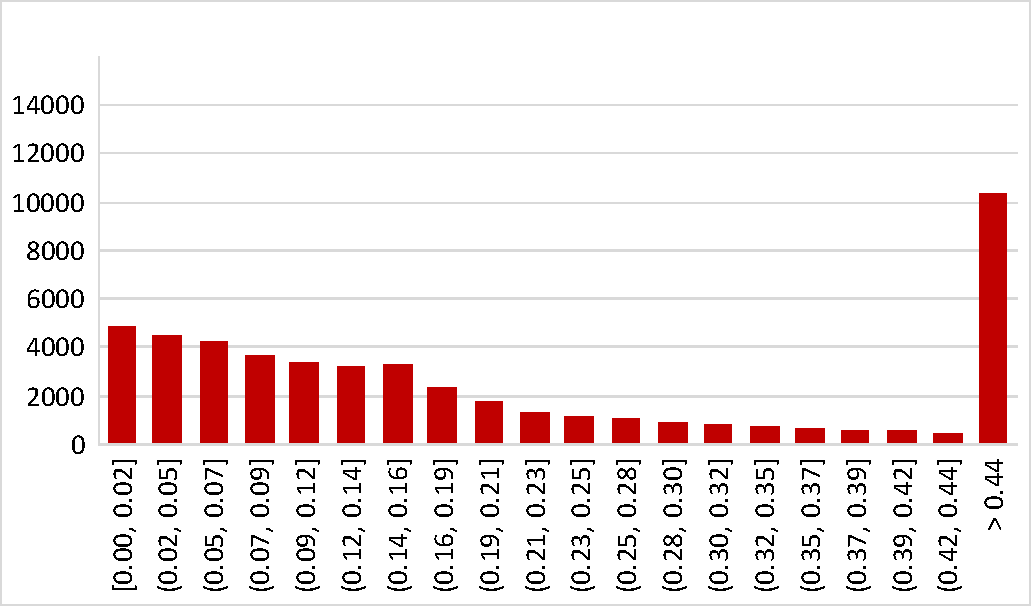
\includegraphics[width=1\linewidth]{results/nyx/Lag100_8_Max.pdf}
%\caption{Lagrangian 100 1:8 Max$_{L2}$}
%\end{subfigure}
%\hspace{1mm}
%\begin{subfigure}{0.20\textwidth}
%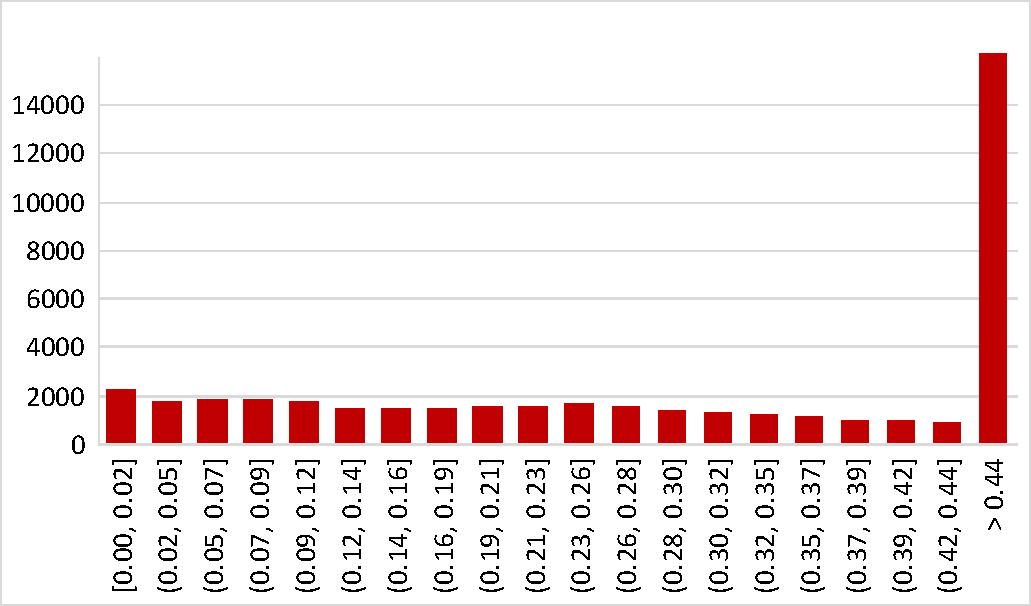
\includegraphics[width=1\linewidth]{results/nyx/Lag100_27_Max.pdf}
%\caption{Lagrangian 100 1:27 Max$_{L2}$}
%\end{subfigure}
%\hspace{1mm}
%\hspace{1mm}
%\begin{subfigure}{0.20\textwidth}
%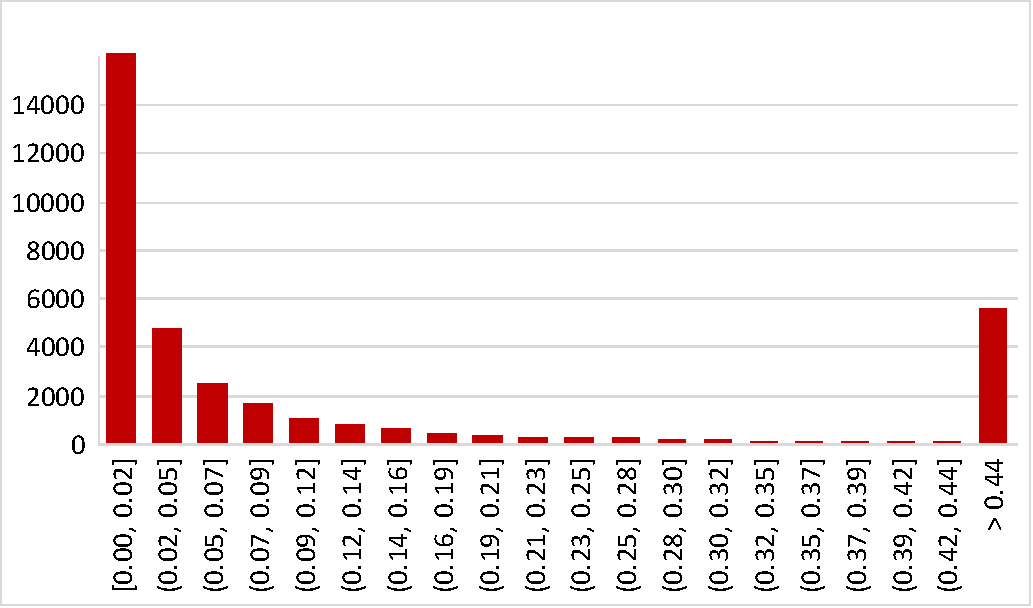
\includegraphics[width=1\linewidth]{results/nyx/Lag200_8_AvgL2.pdf}
%\caption{Lagrangian 200 1:8 Avg$_{L2}$}
%\end{subfigure}
%\hspace{1mm}
%\begin{subfigure}{0.20\textwidth}
%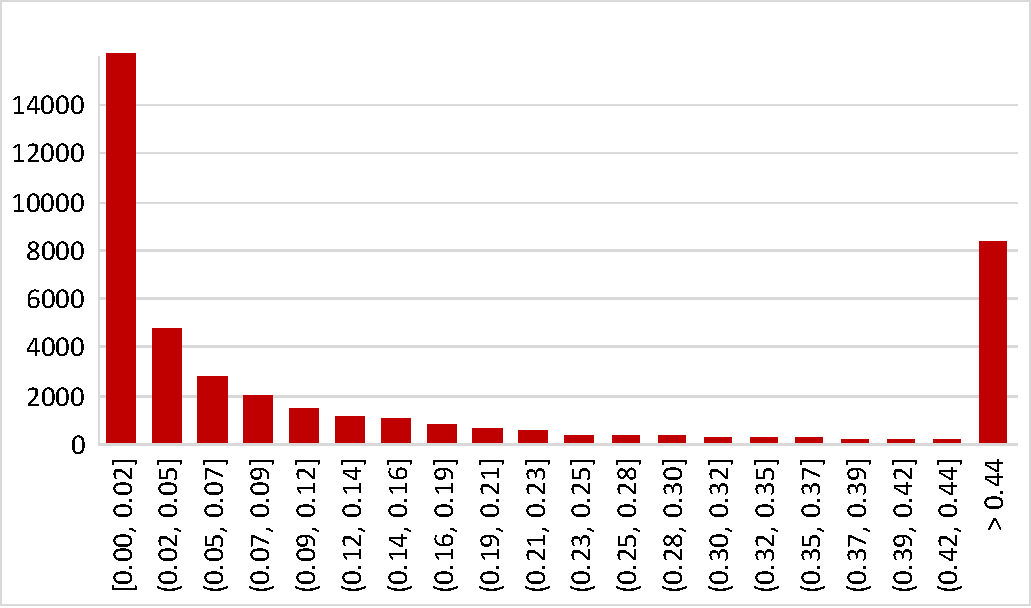
\includegraphics[width=1\linewidth]{results/nyx/Lag200_27_AvgL2.pdf}
%\caption{Lagrangian 200 1:27 Avg$_{L2}$}
%\end{subfigure}
%\begin{subfigure}{0.20\textwidth}
%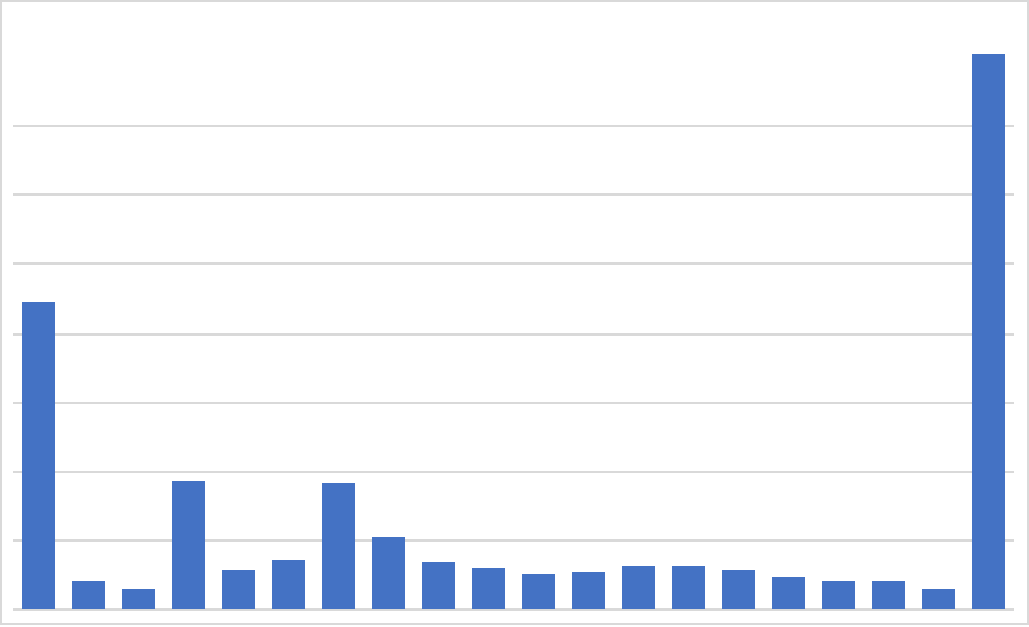
\includegraphics[width=1\linewidth]{results/nyx/Eul200_Max.pdf}
%\caption{Eulerian 200 Max$_{L2}$}
%\end{subfigure}
%\hspace{1mm}
%\begin{subfigure}{0.20\textwidth}
%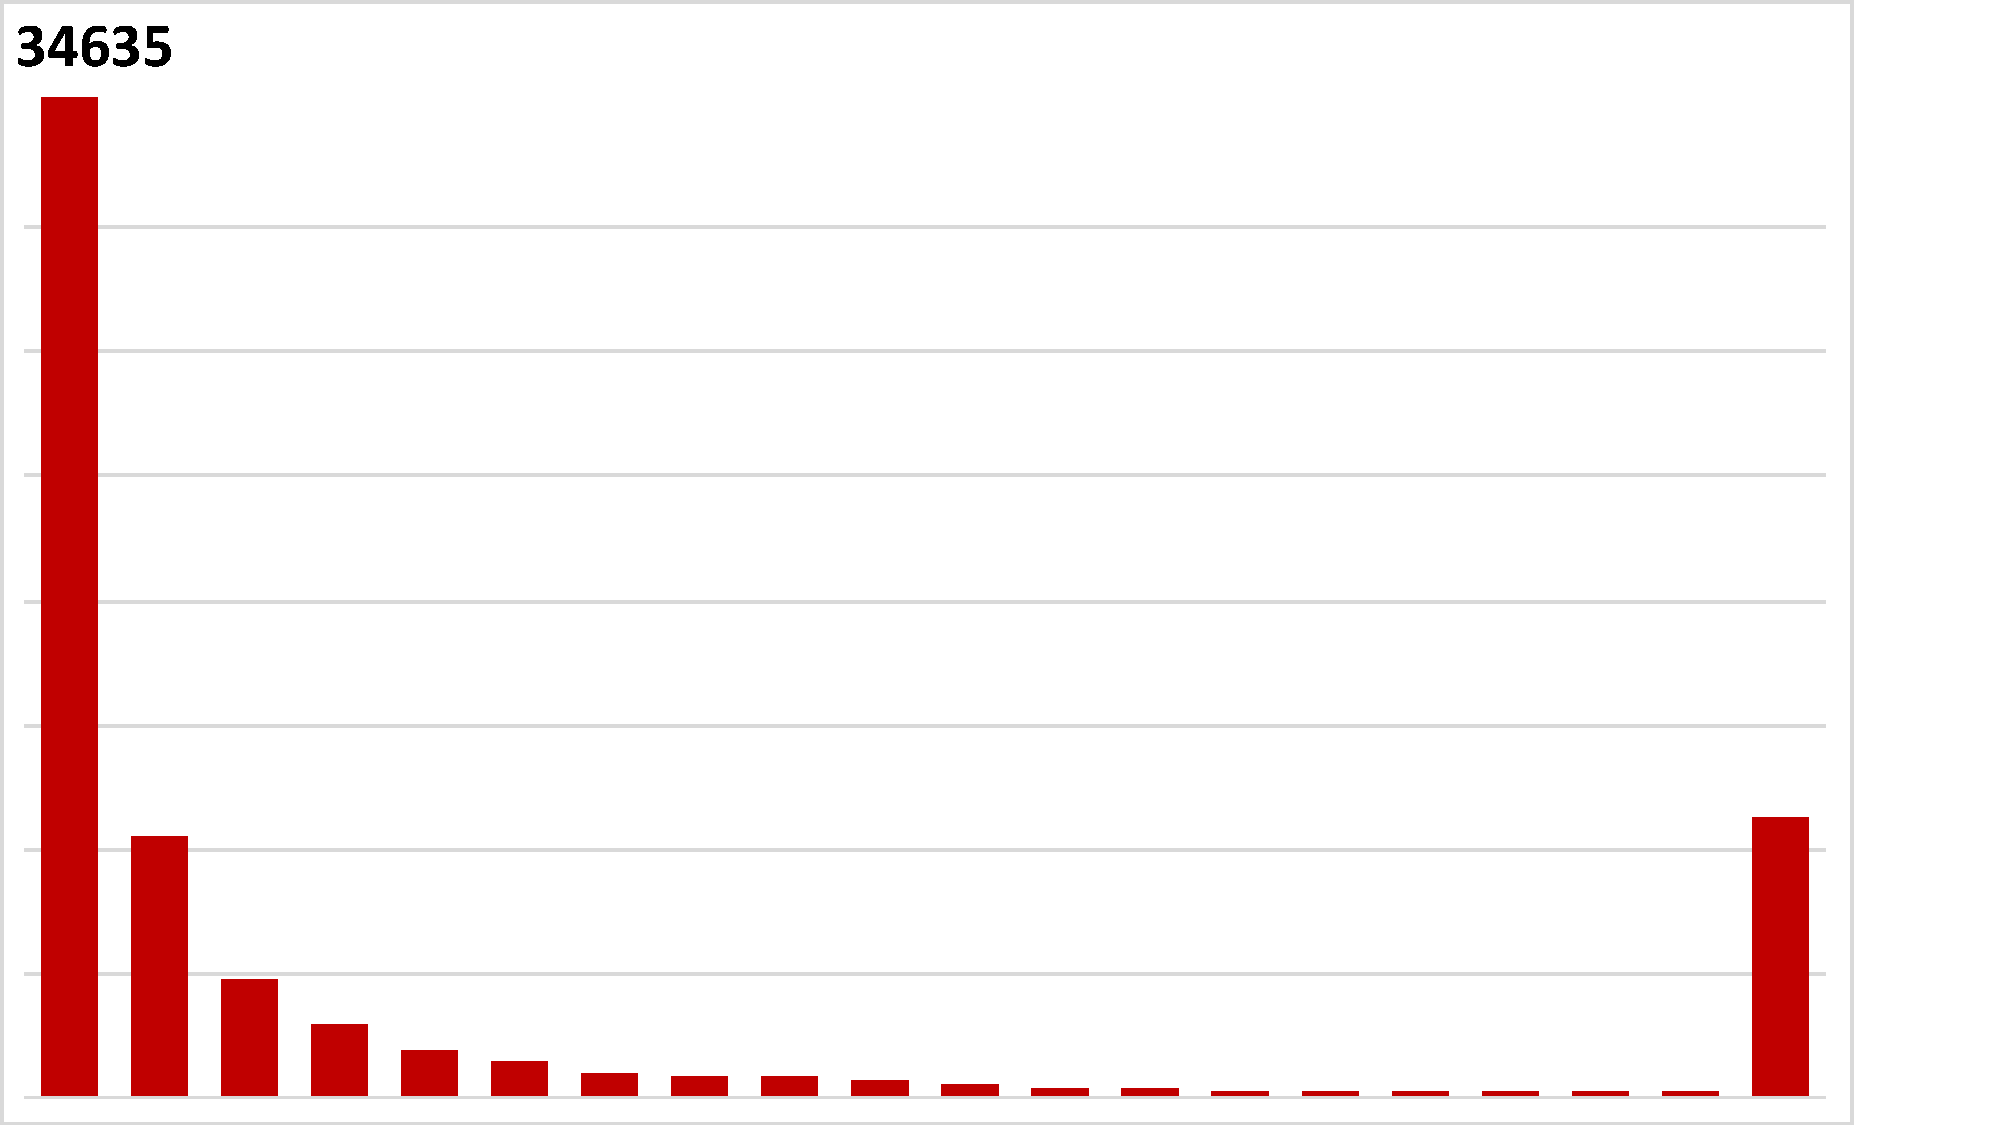
\includegraphics[width=1\linewidth]{results/nyx/Lag200_1_Max.pdf}
%\caption{Lagrangian 200 1:1 Max$_{L2}$}
%\end{subfigure}
%\hspace{1mm}
%\begin{subfigure}{0.20\textwidth}
%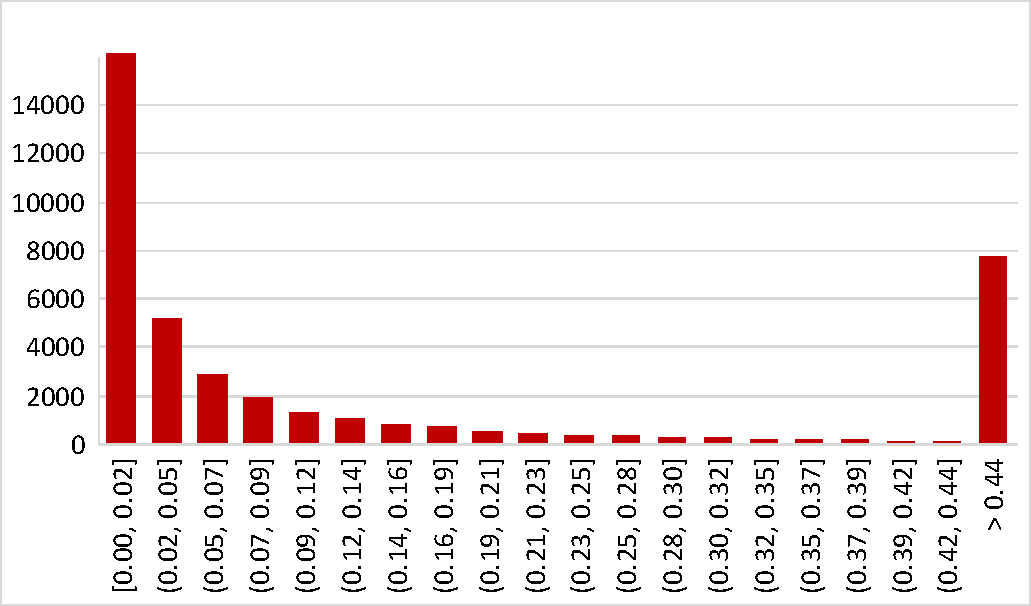
\includegraphics[width=1\linewidth]{results/nyx/Lag200_8_Max.pdf}
%\caption{Lagrangian 200 1:8 Max$_{L2}$}
%\end{subfigure}
%\hspace{1mm}
%\begin{subfigure}{0.20\textwidth}
%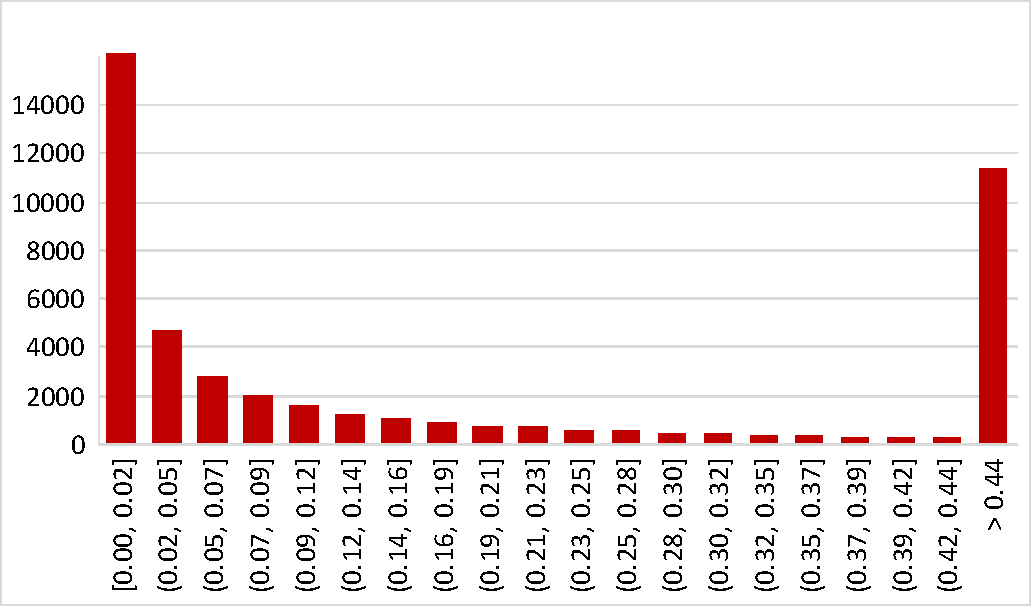
\includegraphics[width=1\linewidth]{results/nyx/Lag200_27_Max.pdf}
%\caption{Lagrangian 200 1:27 Max$_{L2}$}
%\end{subfigure}
\caption{Nyx experiment histograms for 50,000 test particle interpolation errors. Each plot has 20 bins, ranging from 0 to $>$0.44, with bar height encoding number of particles. Horizontal grid lines mark increments of 2,000.}
\label{fig:nyx_hist}
\end{figure*}

